%Sidenote from Angie: Green text after a percentage sign includes notes to the LaTeX code, useful tips and tricks I thought you might need ⁠— feel free to read them for extra info on this template.

%~~~~~~~~~~~~~~~~~~~~~~~~~~~~~~~~~~~~~~~~~~~~~~~~~~~~~~~%
% Changelog 7.21: Lab now moving from remote learning to physical laboratory, please ignore any comments after '% OLD TEXT IGNORE:'
%Changelog 10.21: Fixed the formatting of RSC referencing style 
%Changelog 1.22: Reviewed before the start of Semester 2, fixed some wording/clarification issues
%Changelog 5.22: Reviewed after semester 2, fixed some wording/clarification issues, removed OLD TEXT
%~~~~~~~~~~~~~~~~~~~~~~~~~~~~~~~~~~~~~~~~~~~~~~~~~~~~~~~%

\documentclass[twocolumn]{article} %sets the type of the document that you compile, for just now it is an article - specifically one with a two-column formatting

%~~~~~~~ Packages ~~~~~~~~~%
% Please don't be scared by the chunk of code below, these are just some handy tools that make using LaTeX easier, you can read more on your own time, for example here: https://www.latex-tutorial.com/tutorials/packages/
%\usepackage{amsmath}
% \usepackage{caption}
% \usepackage{subcaption}
\usepackage[utf8]{inputenc} %helps interpret unicode, non ASCII characters
\usepackage[T1]{fontenc} %makes font compatible with more non-ASCII characters
\usepackage[english]{babel} %allows the use of special characters and also translates some elements within the document. This package also automatically activates the appropriate hyphenation rules for the language you choose
\usepackage{ifpdf,amsmath,amsthm,amssymb,amsfonts,newtxtext,newtxmath} %helps formatting math & keeps it looking tidy when compiling PDFs
\usepackage{array,graphicx,dcolumn,multirow,abstract,hanging} %makes tables compile properly & helps with nice table formatting
\usepackage{subcaption}
\usepackage[font={it,footnotesize},labelfont=bf]{caption} %makes captions nicer
\usepackage[hyperfootnotes=false,breaklinks=true,hidelinks]{hyperref} %formats hyperlinks
%\hypersetup{colorlinks=false,} %formats hyperlinks
\usepackage{float} %improves the interface for defining floating objects such as figures and tables
\urlstyle{same} %formats urls
\usepackage{url} %formats urls
\usepackage[version=4]{mhchem} %helps format chemical formulae see more info at https://anorien.csc.warwick.ac.uk/mirrors/CTAN/macros/latex/contrib/mhchem/mhchem.pdf
\usepackage{siunitx} %formats SI units see more info at http://www.bakoma-tex.com/doc/latex/siunitx/siunitx.pdf
\usepackage{color,soul} %allows for highlighting text
\usepackage[super,sort&compress,comma]{natbib}  % use natbib
\setlength{\bibsep}{0pt plus 0.3ex} % set spacing of bibliography
\usepackage{booktabs} % \toprule \midrule \bottomrule \cmidrule(lr){a-b}
%\usepackage{capt-of}
% define centered and ragged columns:
\newcolumntype{L}[1]{>{\raggedright\arraybackslash }p{#1}} % can use m{}
\newcolumntype{C}[1]{>{\centering\arraybackslash }p{#1}}
\newcolumntype{R}[1]{>{\raggedleft\arraybackslash }p{#1}}
\newcolumntype{d}[1]{D{.}{.}{#1}} % d{3.2} for 3 places on l, 2 on r
\newcommand{\mc}{\multicolumn}
\topmargin=-.3in \oddsidemargin=-.1in \evensidemargin=-.1in \textheight=9in \textwidth=6.8in
\setlength\tabcolsep{1mm}
\setlength\columnsep{8mm}
\setlength\abovecaptionskip{.5ex}
\setlength\belowcaptionskip{.5ex}
\setlength\belowbottomsep{.3ex}
\setlength\lightrulewidth{.04em}
\renewcommand\arraystretch{1.2}
\renewcommand{\topfraction}{1}
\renewcommand{\textfraction}{0}
\renewcommand{\floatpagefraction}{.9}
\renewcommand{\thefootnote}{\roman{footnote}}
% \renewcommand{\baselinestretch}{1.00} \large\normalsize % for fixing spaces
\widowpenalty=1000
\clubpenalty=1000
\setlength{\parskip}{0ex}
\let\tempone\itemize
\let\temptwo\enditemize
\let\tempthree\enumerate
\let\tempfour\endenumerate
\renewenvironment{itemize}{\tempone\setlength{\itemsep}{0pt}}{\temptwo}
\renewenvironment{enumerate}{\tempthree\setlength{\itemsep}{0pt}}{\tempfour}
%the above is the formatting setup for keeping the two-column article and tables working nicely, feel free to tinker with it, but I suggest only doing so once you know what you're doing with LaTeX
%~~~~~~~~~~~~~~~~~~~~~~~~~~%

%!!!!!!!!!!!!!!!!!!!!!!!!!!!!!!!!!!!!!!%
% REPORT STARTS HERE %

%\date{} %if you don't want the date to show up in your report, uncomment this (=remove the percentage symbol at the start of the line)
\setcounter{page}{1} % starts counting pages from the first
\title{\textit{Experiment [IRS]:} Determining Molecular Constants with Rotational-VibrationalSpectroscopy} % change to an actual title for your report!
\author{Qianrui Li}

\begin{document}
\twocolumn[ %this command makes your title and abstract both be one column only
\vspace{-.5in}
\maketitle
\centering
\vspace{-0.3in}
\section*{Abstract}
{\large 
The vibrational rotational spectrums of the HCl molecule and cigarette smoke were obtained in this experiment using a Fourier Transform Infrared Spectrometer (FTIR). For the HCl molecule, each peak in the spectrum splited into two peaks because $^{35}$Cl had an isotope, $^{37}$Cl, which was heavier and had lower transition energy. The rotational constant in the ground vibrational state, $B_0$, and first existed state, $B_1$, of HCl$^{35}$ were determined as 10.3488 $\pm$0.0110 cm$^{-1}$ and 10.0456 $\pm$0.0110 cm$^{-1}$ respectively, and were used to calculate the value of $B_e$, which was 10.5003 $\pm$0.0110 cm$^{-1}$. The bond length in different vibrational level ($r_0$, $r_1$, $r_e$), the equilibrium oscillation frequency $\omega_e$, anharmonicity constant $x_e$, zero-point energy G(0), and force constant of HCl$^{35}$ and HCl$^{37}$ were calcualted and compared with the literature value. The difference between the parameters of HCl$^{35}$ and HCl$^{37}$ were disccussed. The spectrum of cigarette smoke was also obtained, and the peaks in the spectrum were assigned to the vibrational rotational transition of CO, CO$_2$, HCN, CH$_4$, and H$_2$O. The values of $B_0$, $B_1$, $B_e$, $r_0$, $r_1$, $r_e$, $\omega_e$, $x_e$, G(0), and force constant of CO were calculated and compared with the value of HCl, and the difference between them was discussed. 

}
\vspace{0.4in}
]
%\setlength{\baselineskip}{12pt plus.2pt}


\section{Introduction} % example of a heading

\textbf{Vibrational Energy}

The vibrational population can be transferred from the ground state to a higher state by absorbing energies. The \textit{fundamental absorption} described the transition from v=0 to v=1, and the energy was usually in the range of 500 cm$^{-1}$ to 4000 cm$^{-1}$, which was within the infrared region. 

The energy levels for diatomic molecules in an anharmonic state could be expressed as shown in equation 1.

\begin{equation}
    G(v) = (v + \frac{1}{2}) \omega_e - (v + \frac{1}{2})^2\omega_ex_e \label{eq.1}
\end{equation}

In the first part of the equation 1 represented the energy of a harmonic oscillator, while the second part was the correction term for an anharmonic oscillator. The energy of an anharmonic oscillator was lower than the energy of a harmonic oscillator with an amount depending on the anharmonic constant $\omega_ex_e$. The frequency of the anharmonic oscillator was shown as $\omega_e$. With equation 1, the ground state energy could be shown as equation 2 with v=0, and so as the first excitation state (v=1) and the second excitation state (v=2).
\begin{subequations}
    \begin{align}
        G(0) = \frac{1}{2}\omega_e - \frac{1}{4}\omega_ex_e \\
        G(1) = \frac{3}{2}\omega_e - \frac{9}{4}\omega_ex_e \\
        G(2) = \frac{5}{2}(\omega_e -\frac{25}{4}\omega_ex_e) 
    \end{align}
\end{subequations}

With equation 2, the energy of the fundamental absorption (v=0 to v=1) and the energy of the first overtone (v=0 to v=2) could be calculated as shown in equation 3. 
\begin{subequations}
    \begin{align}
        G(0 \rightarrow 1) = G(1) - G(0) = \omega_e - 2\omega_ex_e \\
        G(0 \rightarrow 2) = G(2) - G(0) = 2(\omega_e - 3\omega_ex_e) 
    \end{align}
\end{subequations}

\textbf{Rotational Energy}

The rotational energy could be described using equation 4 for a diatomic molecule.

\begin{equation}
    F(J) = B_v(J + 1) \label{eq.4}
\end{equation}

In this equation, $J$ was the rotational quantum number, while $B_v$ was the rotational constant, which was related to the moment of inertia $I$ as shown in equation 5. 

\begin{subequations}
    \begin{align}
        B_v = \frac{h}{8\pi^2cI} \\
        I = \mu r^2
    \end{align}
\end{subequations}



\textbf{Transition Energy}

Since the vibrational transition and the vibrational transition involved two very different frequencies. The energy for vibrational rotational transition could be expressed as equation \ref{S(v,J)}, while the centrifugal distortion was ignored here. 

\begin{equation}
    S(v,J) = (v + \frac{1}{2}) \omega_e - (v + \frac{1}{2})^2\omega_ex_e + B_v(J + 1) 
    \label{S(v,J)}
\end{equation}

The scale of the constant B would change with increasing vibrational state v because the bond length would increase when the molecule vibrates more violently due to the anharmonicity. Since the value of B depended on the bond length, B would be changed in different vibrational state, which could be quantified by the equation \ref{Be}. 

\begin{equation}
    B_v = B_e - \alpha_e(v + \frac{1}{2}) \label{Be}
\end{equation}

In this equation, $B_e$ was the rotational constant for the ground state, while $\alpha_e$ was the anharmonicity constant. \\
\\



\textbf{Rotational Selection Rules}

When there were two transitions, the rotational state J in the lower vibrational state would be denoted as double prime (J''), while the rotational state J in the upper vibrational state would be denoted as prime (J'). 

The transition where $\Delta J=0$ was forbidden, meaning that transition from J''=1 to J'=1 was not allowed. For $\Delta J=1 $ was allowed and would be shown in the spectrum. The P, Q, R branches were defined based on $\Delta J$:

% The transition where $\Delta J = 0$ was forbidden, meaning that transition from $J=1$ to $J' = 1$ was not allowed. For $\Delta J = 1 $ was allowed and would be shown in the spectrum. The P, Q, R branches were defined based on $\Delta J$:

\begin{enumerate}
    \item P branch - A transition where $\Delta$J=-1, for example, J''=1 to J'=0.
    \item Q branch - A transition where $\Delta$J=0, for example, J''=1 to J'=1.
    \item R branch - A transition where $\Delta$J=+1, for example, J''=1 to J'=2.
\end{enumerate}

% \hl{The Q branch usually would not appeared in the spectrum because it was forbidden (photon unit energy). 
% However, it could appear in the spectrum when ...}

From equation \ref{S(v,J)}, the energy of any rotational state J'' in the ground vibrational state v=0 and the energy of rotational state J' in v=1 could be deduced as shown in equation \ref{S(0to1)}.

\begin{subequations}
    \label{S(0to1)}
    \begin{gather}
        S(0,J^{\prime \prime}) = \frac{1}{2}\omega_e - \frac{1}{4}\omega_ex_e + B_0(J + 1) \label{dp}\\
        S(1,J^{\prime}) = \frac{3}{2}\omega_e - \frac{9}{4}\omega_ex_e + B_1(J + 1) \label{sp}
    \end{gather}
\end{subequations}

Therefore, the transition energy from J'' to J' could be calculated by subtracting equation \ref{dp} from equation \ref{sp} as shown in equation \ref{dptosp}

\begin{equation}
    S(0,J^{\prime \prime} \rightarrow 1,J^{\prime}) = \omega_e - 2\omega_ex_e + (B_1 - B_0)(J + 1) \label{dptosp}
\end{equation}

In an R-branch, $\Delta J = +1$, so J' = J'' + 1. Therefore, the transition energy for an R-branch could be calculated as shown in equation \ref{R} based on equation \ref{dptosp}.In the following equation, J'' was written as J for simplicity.

\begin{equation}
    S(R(J)) = \omega_e - 2\omega_ex_e + B_1(J+1)(J+2) - B_0 J(J+1) \label{R}
\end{equation}

In a P-branch, $\Delta J = -1$, so J' = J'' - 1. Therefore, the transition energy for an P-branch could be calculated as shown in equation \ref{P} based on equation \ref{dptosp}.

\begin{equation}
    S(P(J)) = \omega_e - 2\omega_ex_e + B_1J(J-1)-B_0 J(J+1) \label{P}
\end{equation}

The rotational constant $B_0$ and $B_1$ could be calculated respectively based on equation \ref{R} and \ref{P} as shown in equation \ref{Bv}. 

\begin{subequations}
    \label{Bv}
    \begin{gather}
        S(R(J)) - S(P(J)) = 4 B_1(J+1/2) \\
        S(R(J)) - S(P(J+2)) = 4 B_0(J+3/2)
    \end{gather}
\end{subequations}

These equations were linear, and the value of $B_0$ and $B_1$ could be obtained by plotting the R(J)-P(J) against (J+1/2) and R(J)-P(J+2) against (J+3/2) respectively. The slope of the plot was four times the rotational constant $B_0$ and $B_1$.


% \begin{subequations}
%     % \label{S(0to1)}
%     \begin{align}
%         a=1\\
%         b=1
%         % S(0,J'') = \frac{1}{2}\omega_e - \frac{1}{4}\omega_ex_e + B_0(J'' + 1) \\
%         % S(1,J') = \frac{3}{2}\omega_e - \frac{9}{4}\omega_ex_e + B_1(J' + 1)
%     \end{align}
% \end{subequations}




\section{Methodology}

The 10 $cm^3$ gas cell was flushed with nitrogen and sealed with the Teflon lids. The background scan was performed with this cell using FT-IR spectrometer in the range 6000 cm$^{-1}$ - 2000 cm$^{-1}$ for 64 folds with resolution as 0.5. Three drops of concentrated HCl were added into the cell, and the spectrum was recorded under the same conditions. 

The background scan was performed again under the same conditions with a larger gas cell. Cigarette smoke was captured in the cell using a tube to transform. The spectrum of cigarette smoke was recorded under the same conditions. 


\section{Results}  

The IR sepctrum of HCl was recorded. The fundamental absorption of HCl$^{35}$ was observed at 2885.76 cm$^{-1}$, while the first overtone was observed at 5667.57 cm$^{-1}$. The fundamental absorption of HCl$^{37}$ was observed at 2883.51 cm$^{-1}$, while the first overtone was observed at 5665.32 cm$^{-1}$. The spectrum of HCl were shown in Figure 1.\\[2\baselineskip]

\begin{figure}[h!]
    \begin{subfigure}[b]{0.95\columnwidth}
        %\centering
        %\caption{1a}
        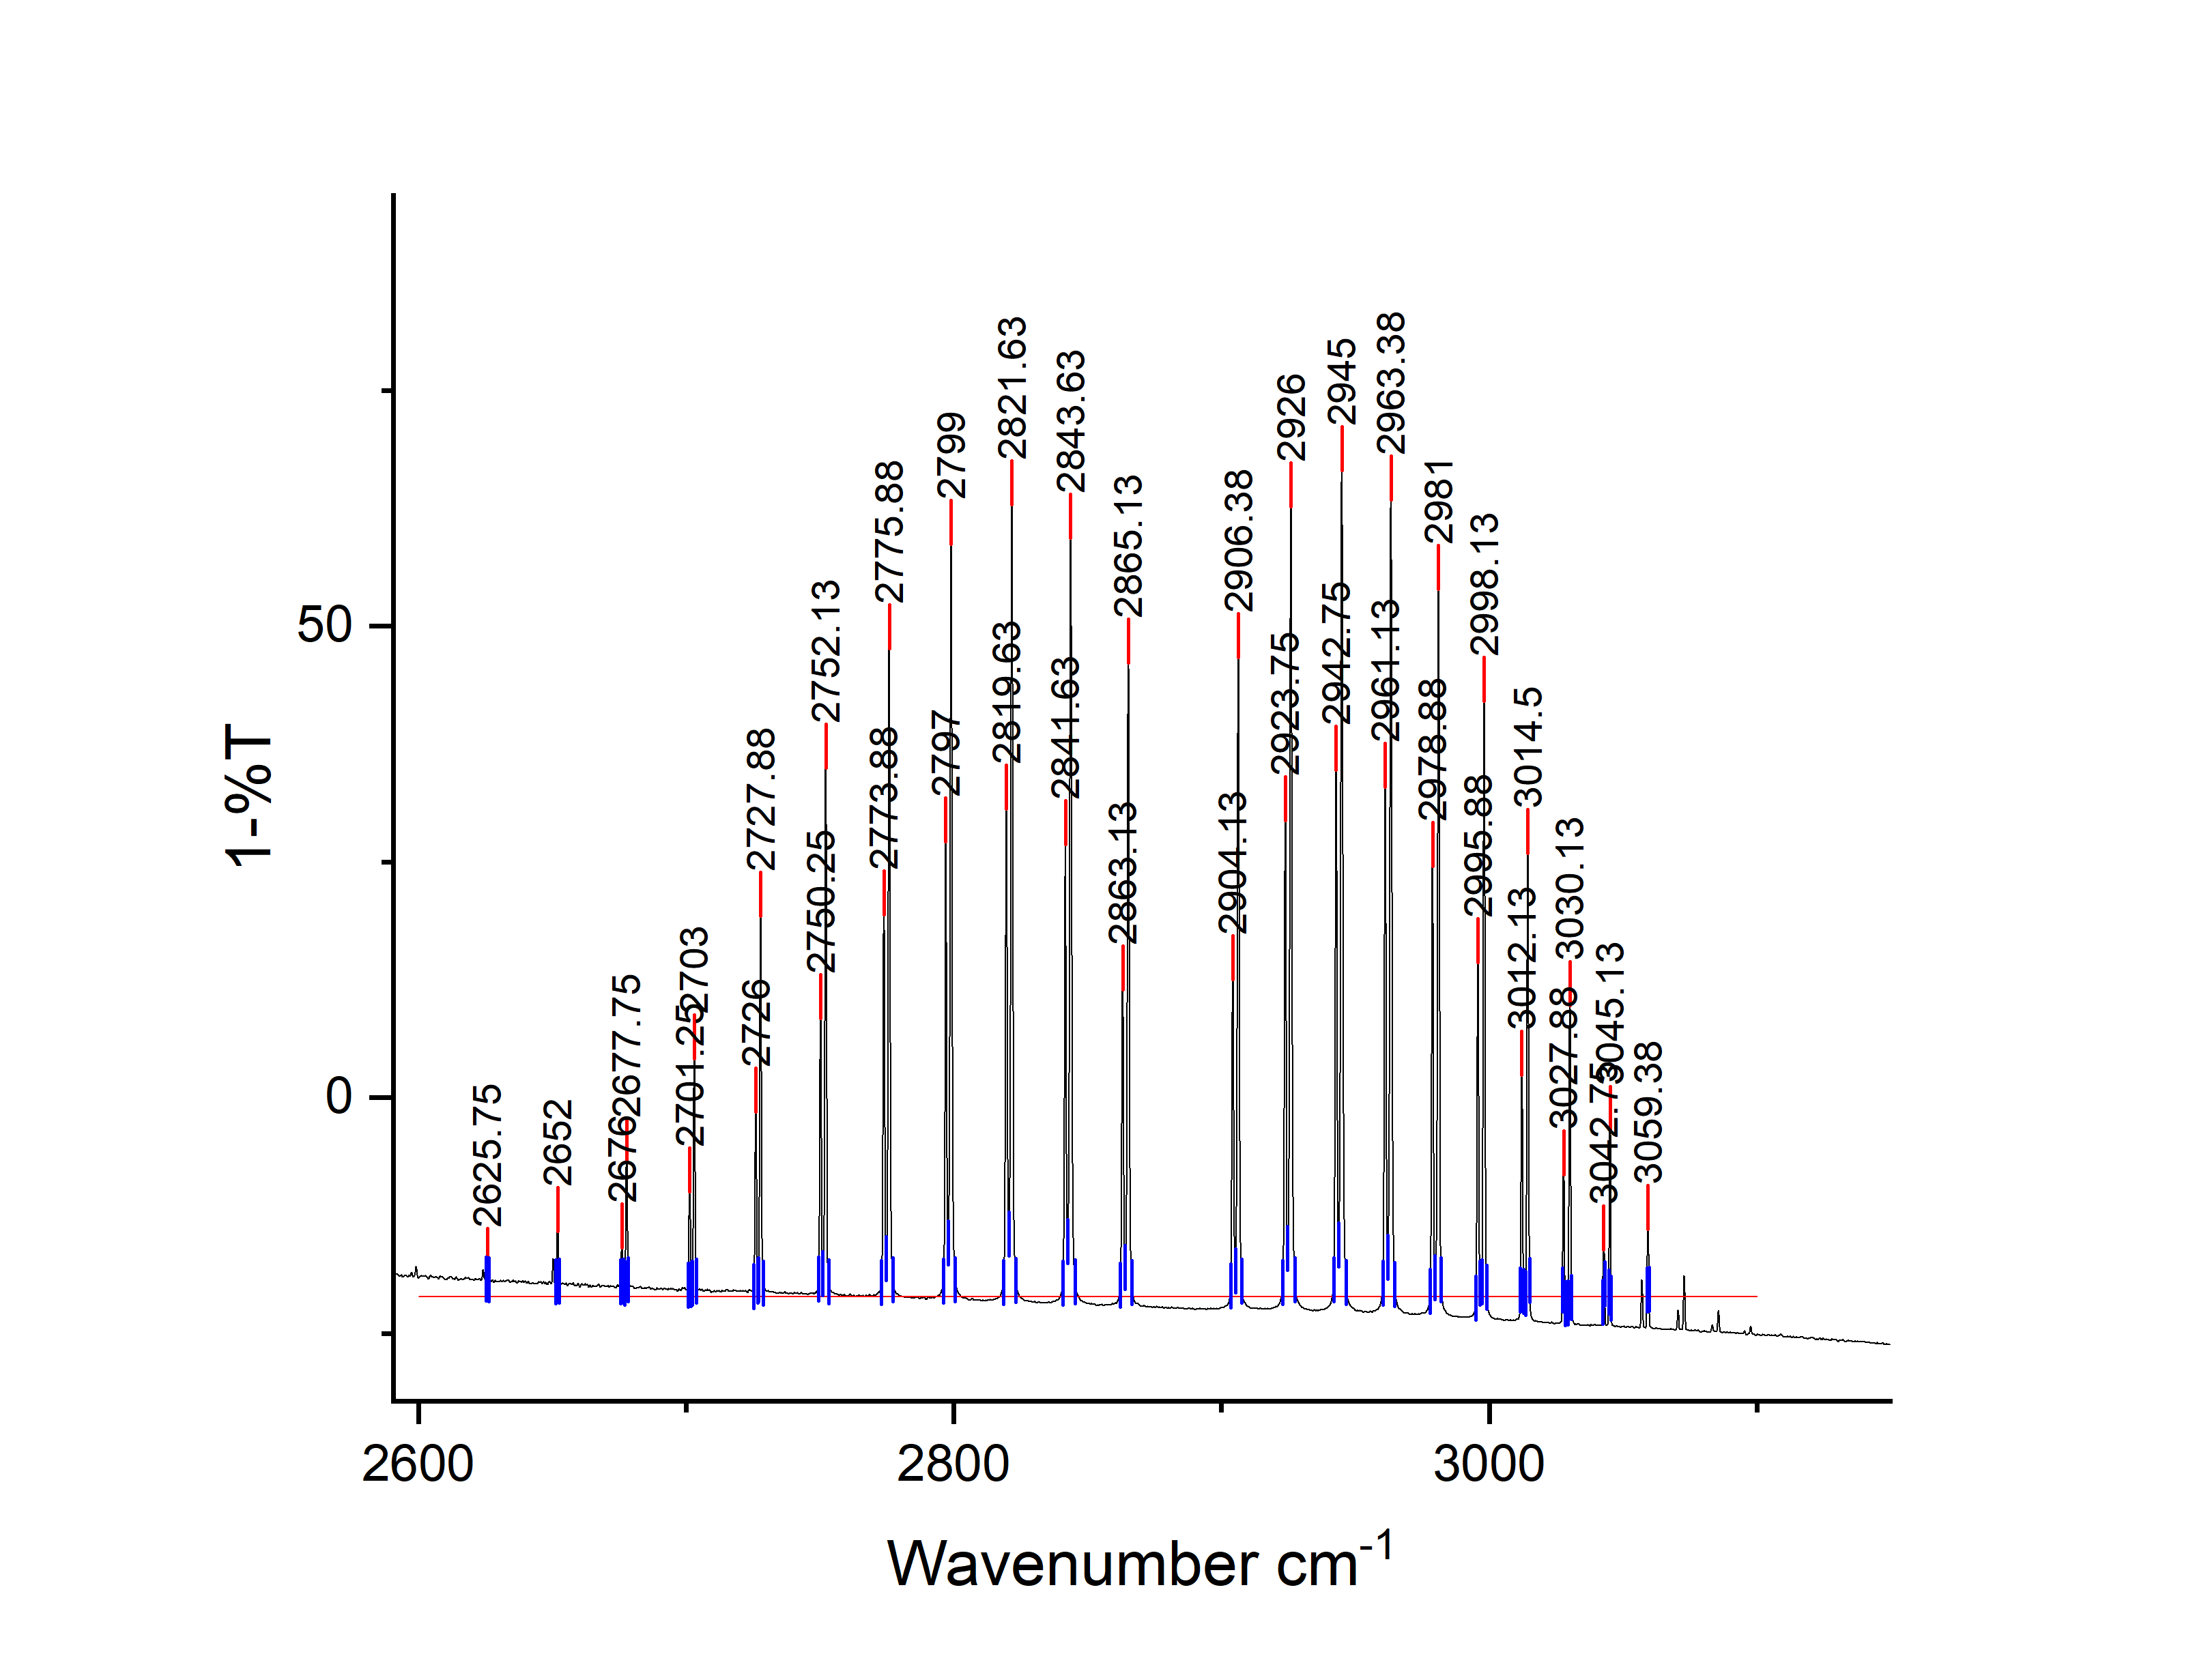
\includegraphics[width=\columnwidth]{HCl fund.png}
        \caption{Fundamental absorption.}
        \label{fig:sfig1}
    \end{subfigure}
    \begin{subfigure}[b]{0.95\columnwidth}
      %\centering
      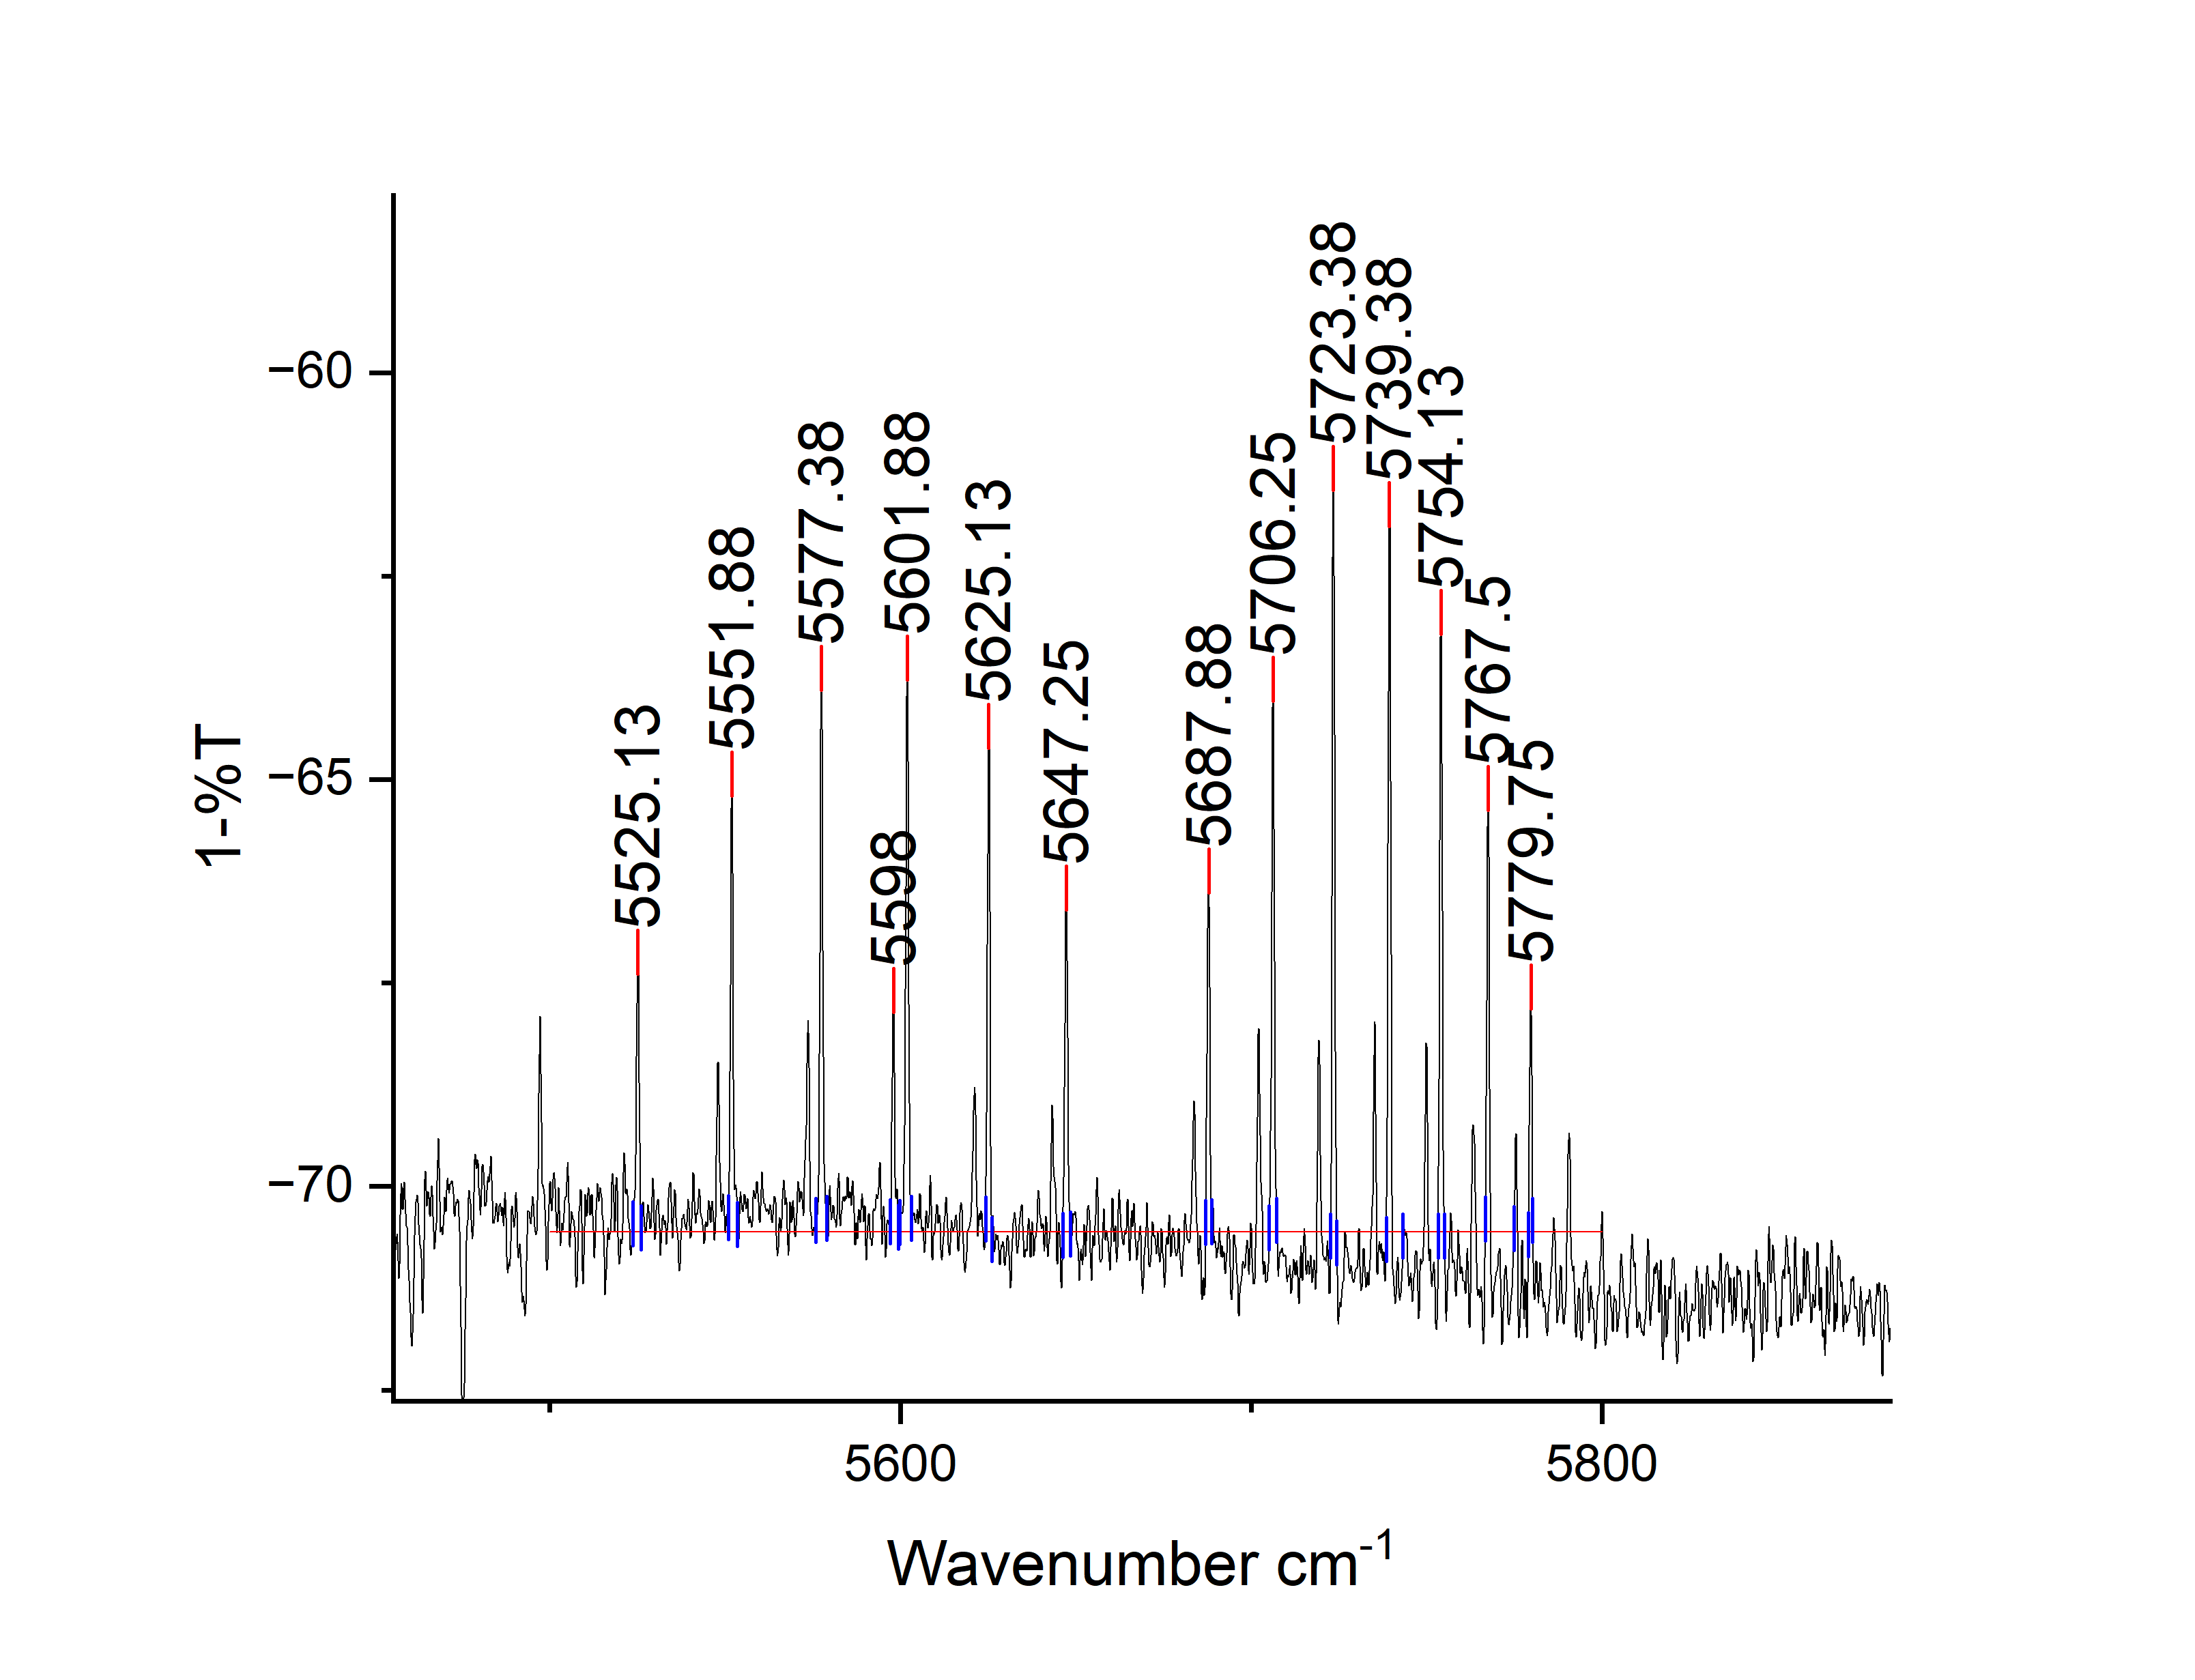
\includegraphics[width=\columnwidth]{HCl over.png}
      \caption{First overtone.}
      \label{fig:sfig2}
    \end{subfigure}
    \caption{The IR spectrum of HCl. The plot (a) was the fundamental absorption, while (b) was the first overtone.}
    %\label{fig:fig}
\end{figure}

Since the P branch had a lower transition energy than the R branch, The peak  with lower wavenumber would be P branch, while the peak with larger peak would be the R branch. \\[2\baselineskip]

The wavenumber of the fundamental absorption for HCl$^{35}$ and HCl$^{37}$ were recorded separately in Table 1 and Table 2. The value of R(J)-P(J) and R(J)-P(J+2) were calculated to determine the rotational constant $B_0$ and $B_1$ for HCl$^{35}$ and HCl$^{37}$ respectively as shwon in Table 1 and Table 2.\\[1\baselineskip]

\begin{table}[h]
    \caption{The wavenumber of the fundamental absorption for HCl$^{35}$ in P branch and R branch.}
    \begin{tabular}{L{.1in}C{.7in}C{.7in}C{.7in}C{.8in}}\toprule
        J & P (cm$^{-1}$)      & R     (cm$^{-1}$)  & R(J)-P(J) (cm$^{-1}$)& R(J)-P(J+2) (cm$^{-1}$)\\\midrule
        0 &     -   & 2906.38 &     -     & 62.75       \\
        1 & 2865.13 & 2926.00 & 60.87     & 104.37      \\
        2 & 2843.63 & 2945.00 & 101.37    & 146.00      \\
        3 & 2821.63 & 2963.38 & 141.75    & 187.50      \\
        4 & 2799.00 & 2981.00 & 182.00    & 228.87      \\
        5 & 2775.88 & 2998.13 & 222.25    & 270.25      \\
        6 & 2752.13 & 3014.50 & 262.37    & 311.50      \\
        7 & 2727.88 & 3030.13 & 302.25    & 352.38      \\
        8 & 2703.00 & 3045.13 & 342.13    &   -          \\
        9 & 2677.75 &     -   &    -      &    - \\\bottomrule
   \end{tabular}
\end{table}

\begin{table}[h]
    \caption{The wavenumber of the fundamental absorption for HCl$^{37}$ in P branch and R branch.}
    \begin{tabular}{L{.1in}C{.7in}C{.7in}C{.7in}C{.8in}}\toprule
        J & P (cm$^{-1}$)      & R     (cm$^{-1}$)  & R(J)-P(J) (cm$^{-1}$)& R(J)-P(J+2) (cm$^{-1}$)\\\midrule
        0 & - & 2904.13 &       -   & 62.50       \\
        1 & 2863.13 & 2923.75 & 60.62     & 104.12      \\
        2 & 2841.63 & 2942.75 & 101.12    & 145.75      \\
        3 & 2819.63 & 2961.13 & 141.50    & 187.25      \\
        4 & 2797.00 & 2978.88 & 181.88    & 228.63      \\
        5 & 2773.88 & 2995.88 & 222.00    & 269.88      \\
        6 & 2750.25 & 3012.13 & 261.88    & 310.88      \\
        7 & 2726.00 & 3027.88 & 301.88    & 351.88      \\
        8 & 2701.25 & 3042.75 & 341.50    &    -    \\
        9 & 2676.00 &     -   &    -      &    - \\\bottomrule
    \end{tabular}
\end{table}

The rotational constant $B_0$ could be obtained by plotting the R(J)-P(J) against (J+1/2) based on equation 12(a) as shown in Figure 2(a) for HCl$^{35}$. The rotational constant $B_1$ could be obtained by plotting the R(J)-P(J+2) against (J+3/2) based on equation 12(b)as shown in Figure 2(b) for HCl$^{35}$. 

\begin{figure}[h!]
    \begin{subfigure}[b]{0.95\columnwidth}
        %centering
        %\caption{1a}
        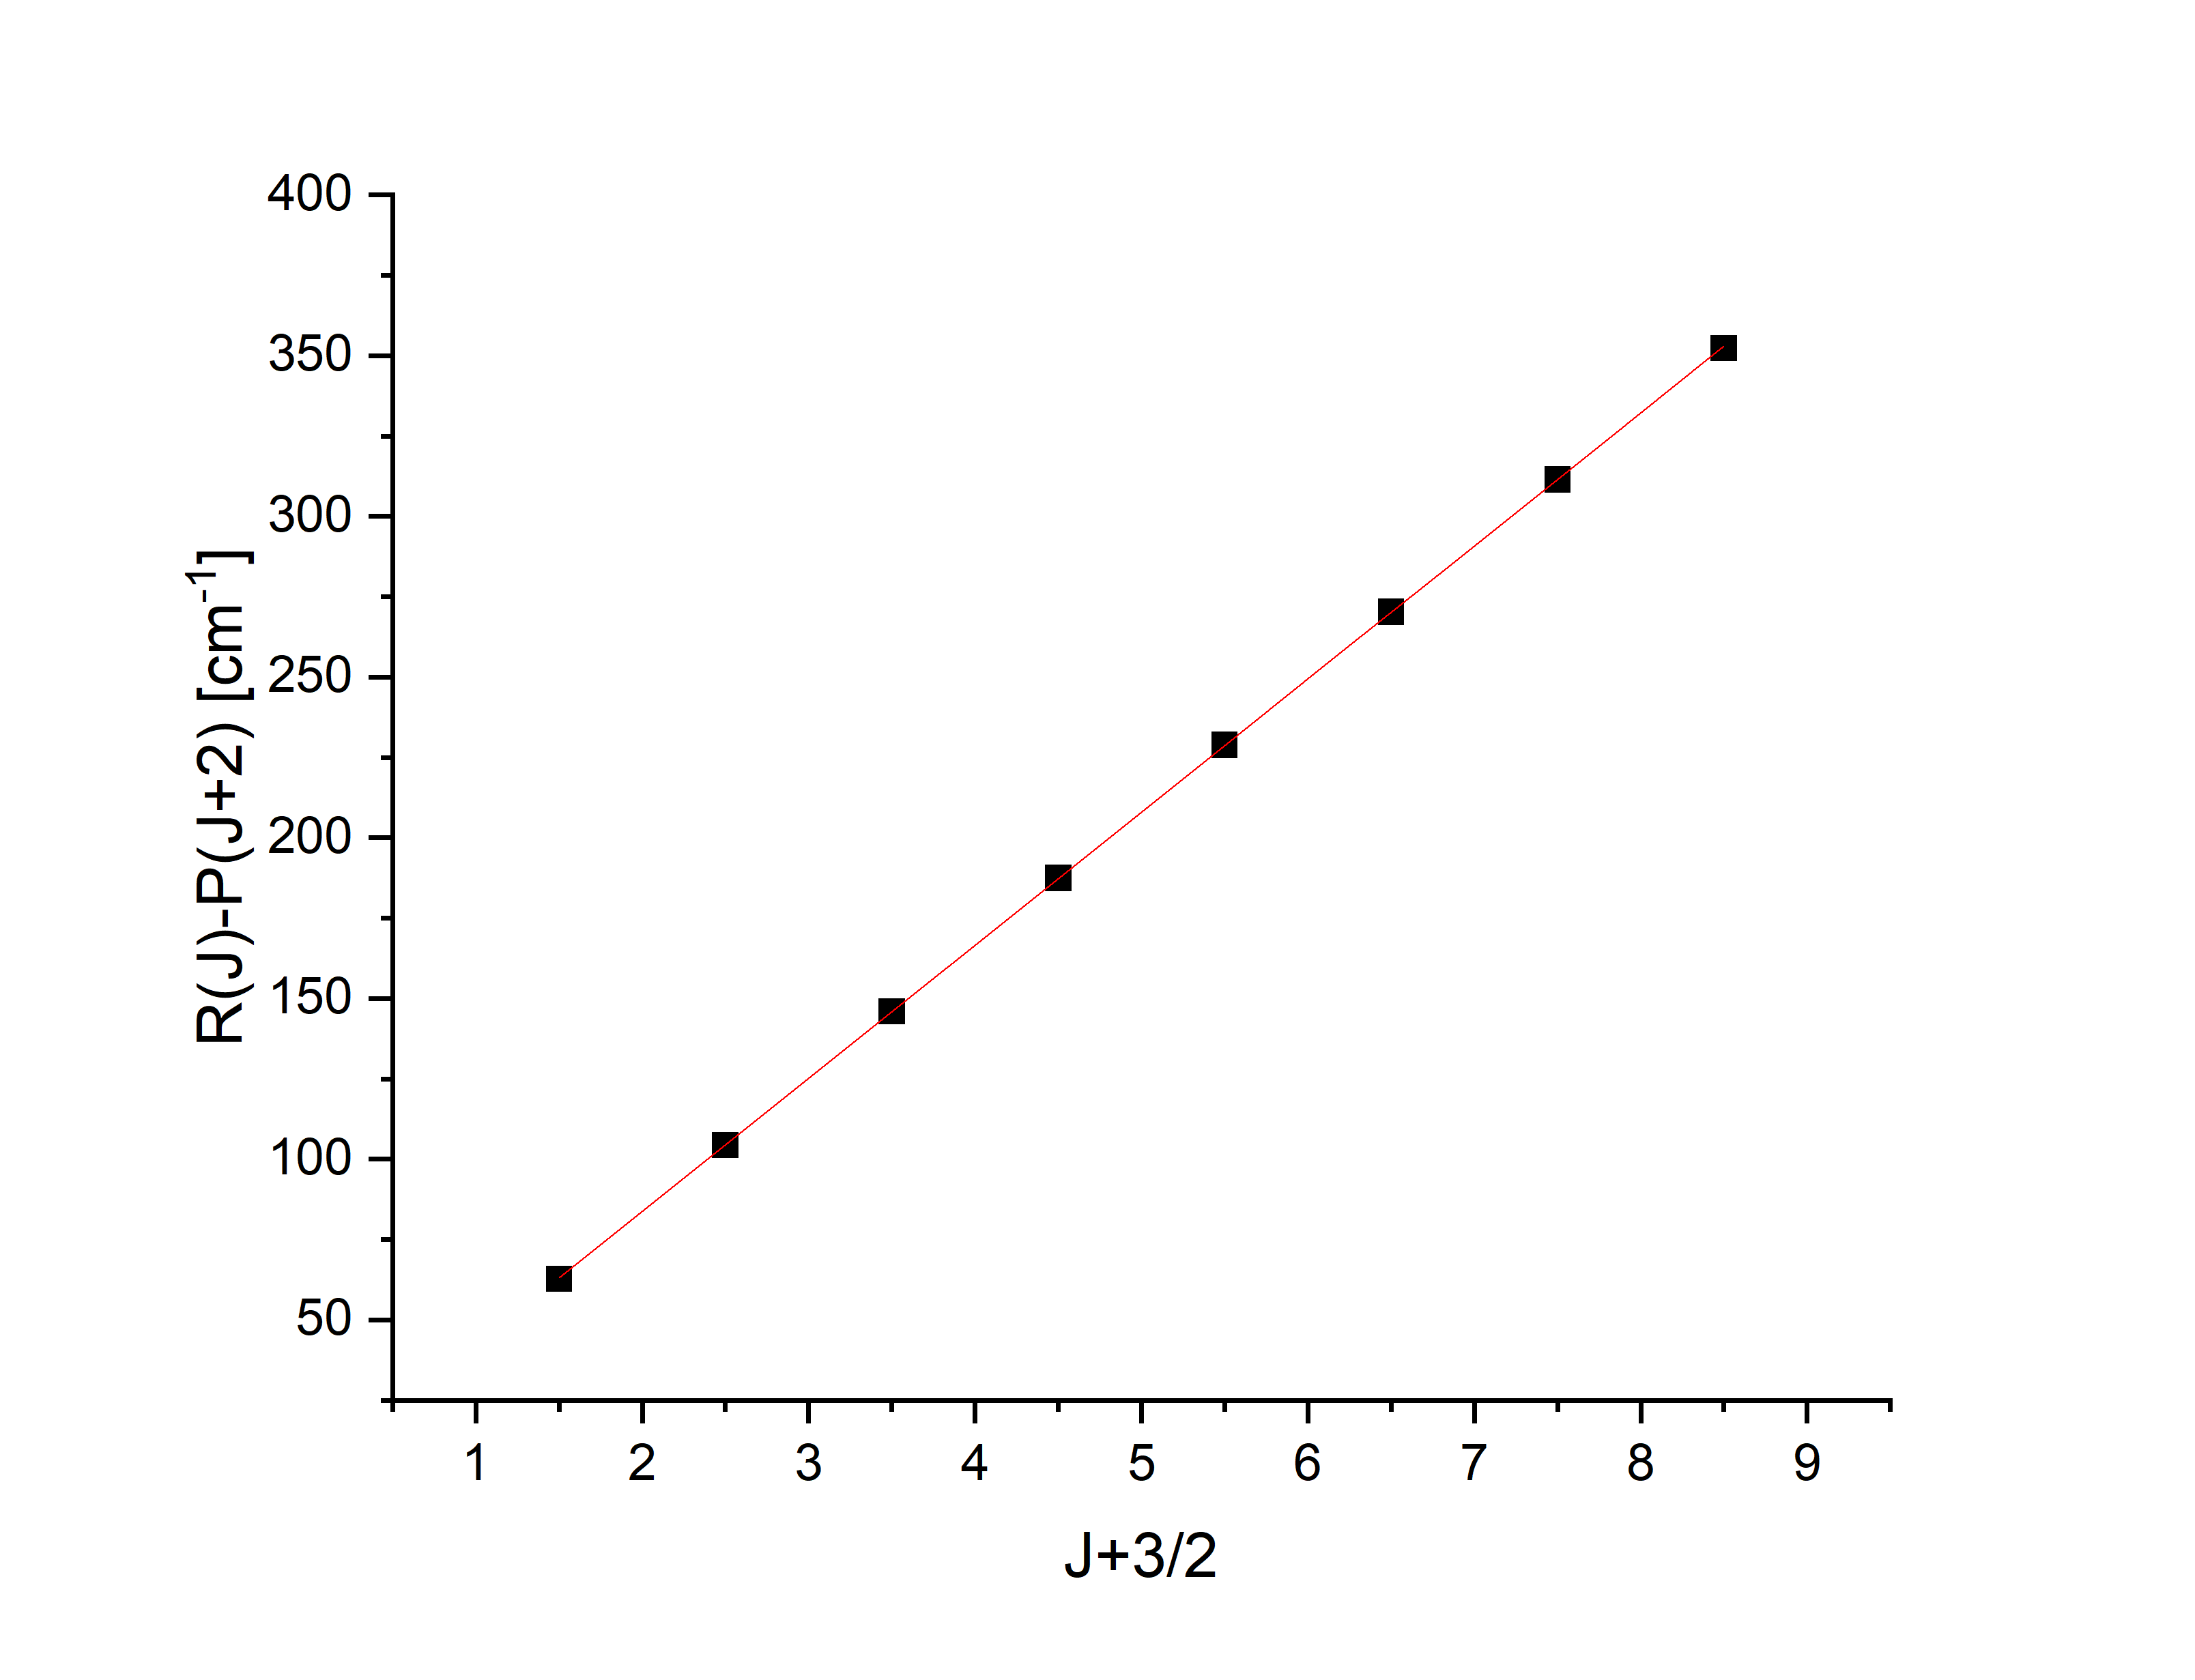
\includegraphics[width=\columnwidth]{HCl-35-B0.png}
        \caption{R(J)-P(J+2) was plotted against (J+3/2).}
        \label{fig:sfig1}
    \end{subfigure}
    \begin{subfigure}[b]{0.95\columnwidth}
      %\centering
      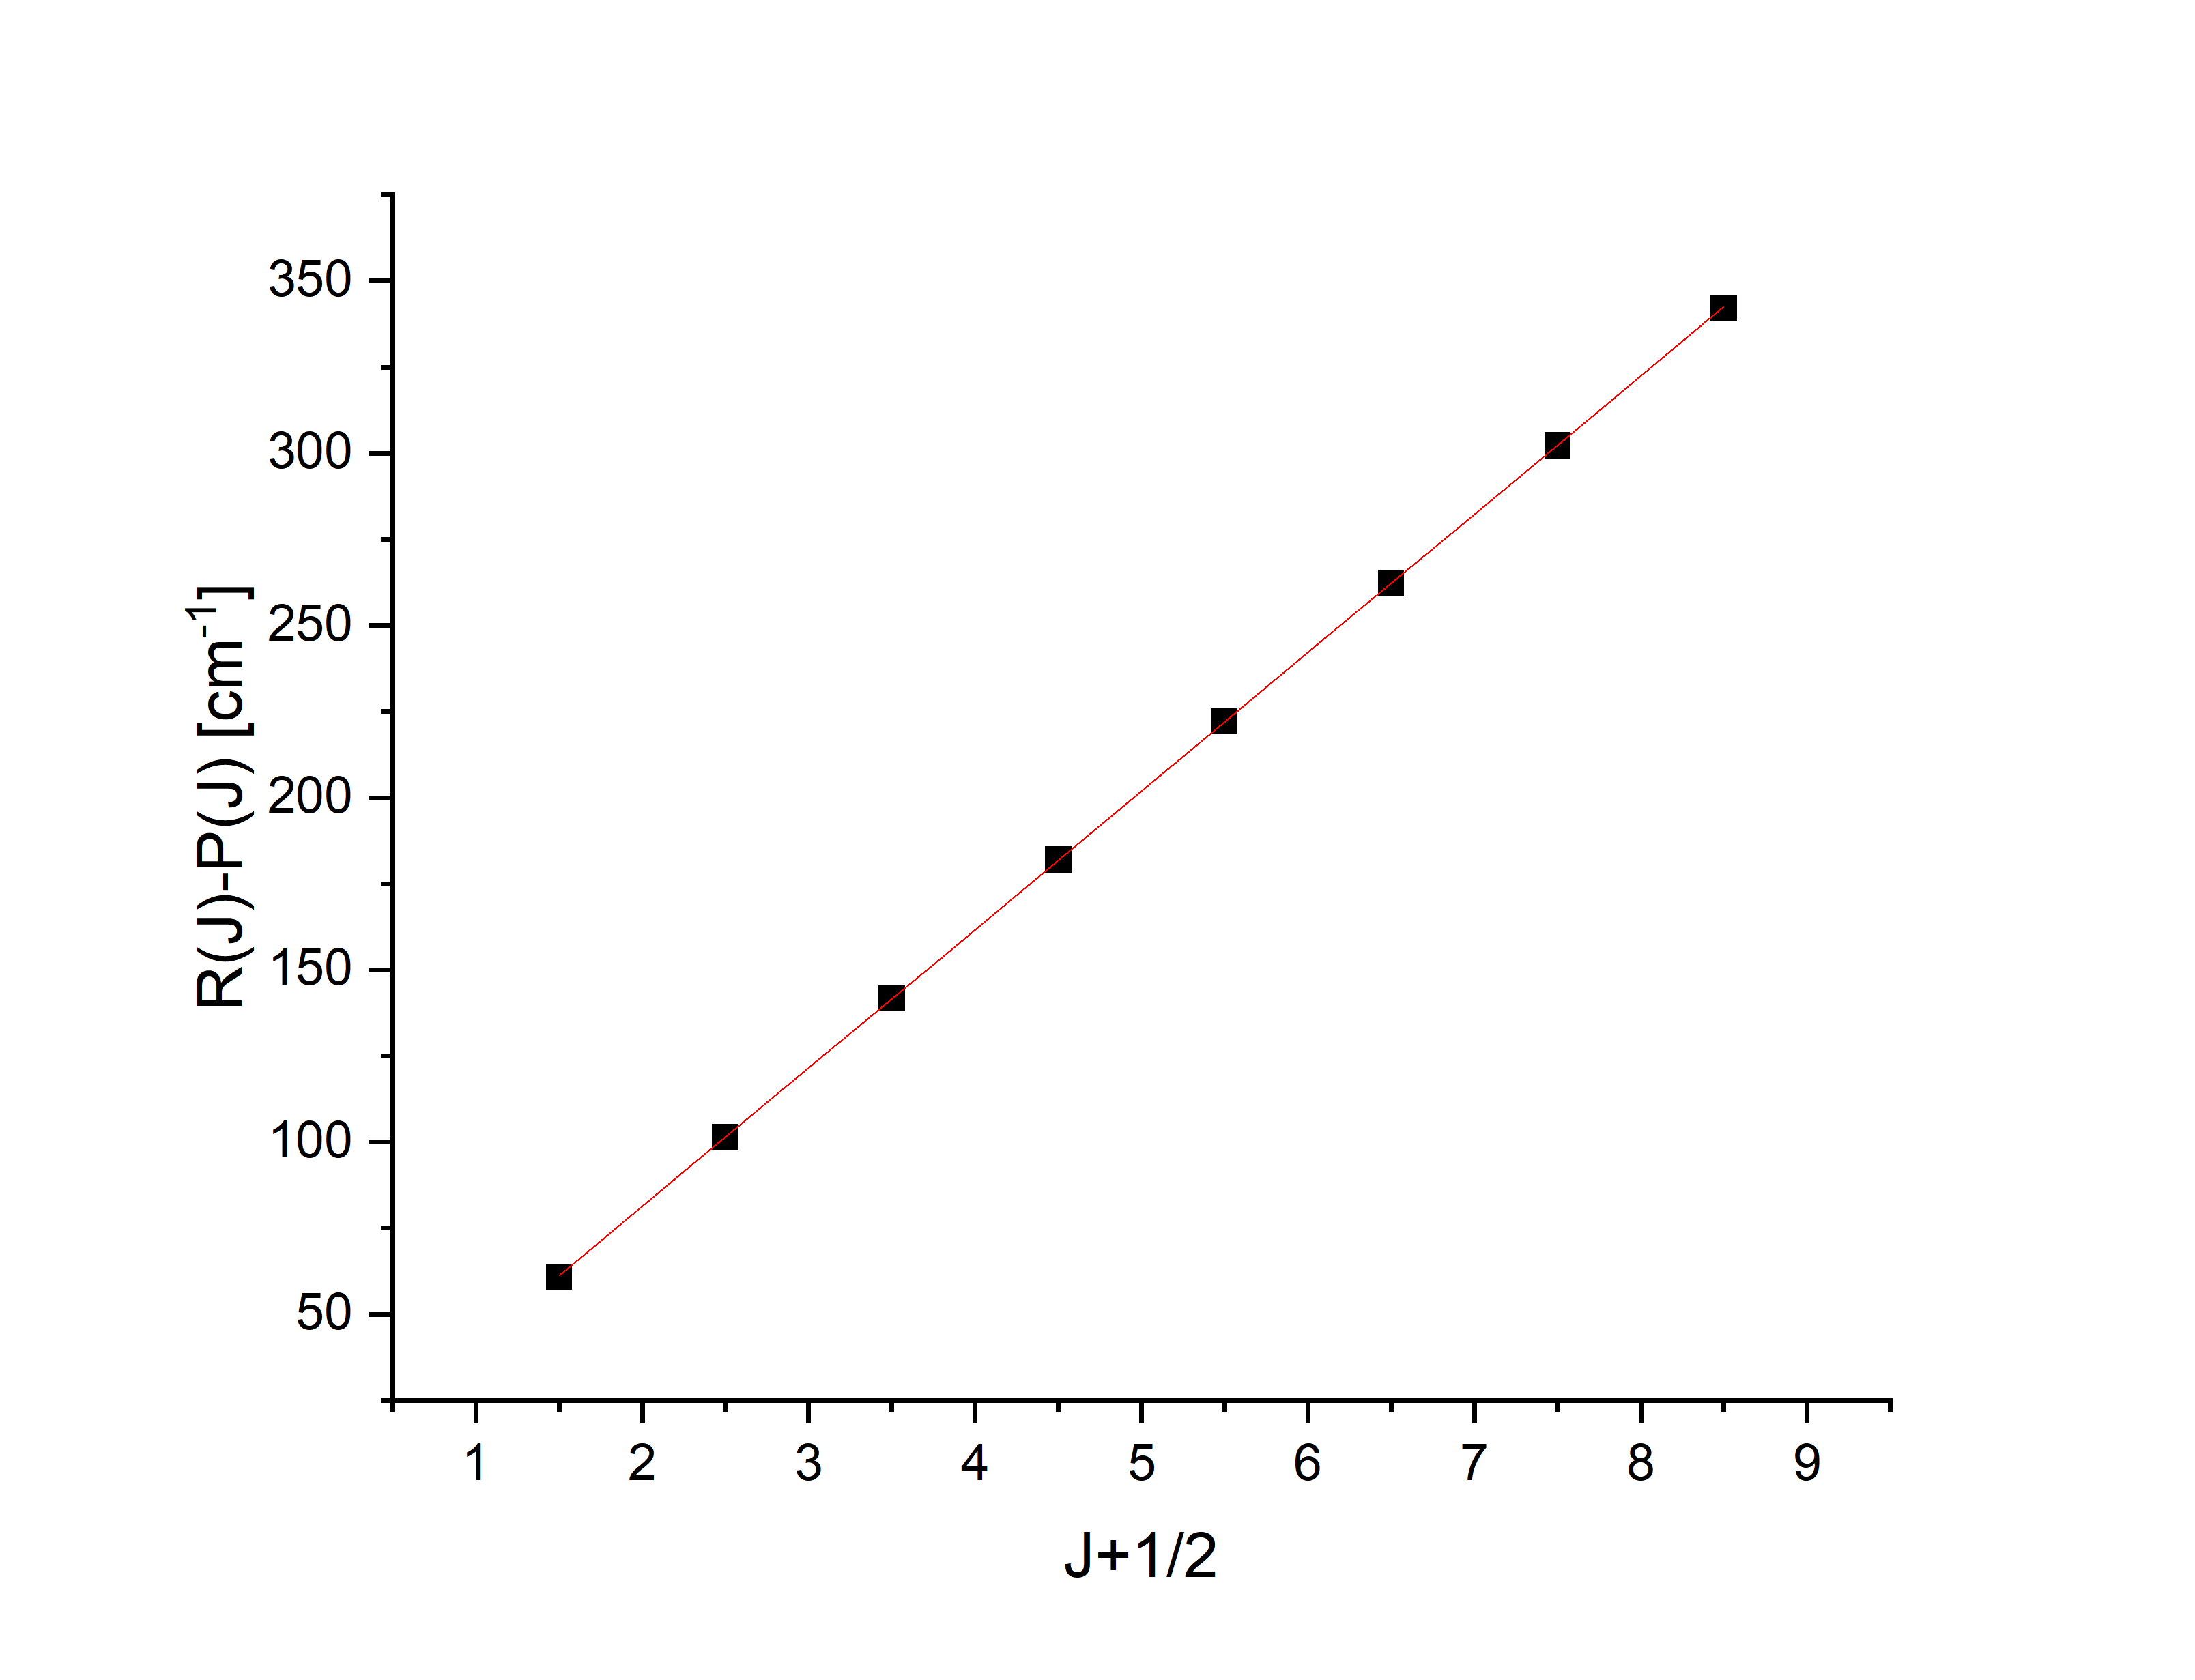
\includegraphics[width=\columnwidth]{HCl-35-B1.png}
      \caption{R(J)-P(J) was plotted against (J+1/2).}
      \label{fig:sfig2}
    \end{subfigure}
    \caption{The rotational constant $B_0$ and $B_1$ for HCl$^{35}$ were calculated based on the slope of the plot. The slope of plot (a) was 41.3950 $\pm$0.0442 with r$^2$ = 1, which was four times the rotational constant $B_0$. The slope of plot (b) was 40.1825 $\pm$0.0440 with r$^2$ = 0.99, which was four times the rotational constant $B_1$.}
    %\label{fig:fig}
\end{figure}

The slope in Figure 2(a) was was four times the rotational constant $B_0$, which was calculated as shown in equation \ref{B_0}.
\begin{equation}
    B_0 = \frac{41.3950 \pm 0.0442}{4} = 10.3488 \pm 0.0110 cm^{-1}
    \label{B_0}
\end{equation}

The slope in Figure 2(b) was four times the rotational constant $B_1$, which was calculated as shown in equation \ref{B_1}.
\begin{equation}
    B_1 = \frac{40.1825 \pm 0.0440}{4} = 10.0456 \pm 0.0110 cm^{-1}
    \label{B_1}
\end{equation}

The rotational constant at equation, $B_e$, could be calculated based on $B_0$ and $B_1$ as shown in equation \ref{B_e} based on equation \ref{Be}.

\begin{subequations}
    \label{B_e}
    \begin{align}
        10.3488 = B_e - \alpha_e (0+1/2)\\
        10.0456 = B_e - \alpha_e (1+1/2)
    \end{align}
\end{subequations}

The value of $B_e$ was determined by solving these two equations, which was 10.5003 $\pm$0.0110 $cm^{-1}$. The value of $\alpha_e$ was also obtained as 0.3029 $cm^{-1}$.

The bond length of HCl in different vibrational could be caluclated using $B_0$, $B_1$, and $B_e$ based on equation 5 respectively as shown in equation \ref{rv}. 


\begin{subequations}
    \label{rv}
    \begin{gather}
        %r =\sqrt{(\frac{h}{8\pi^2\mu B c})}\\
        \mu = \frac{m_H m_{^{35}Cl}}{m_{H}+m_{^{35}Cl}} = 1.6266 \times 10^{-27} kg\\
        r_0 = \sqrt{(\frac{h}{8\pi^2\mu B_0 c})} = 129.0 pm\\
        r_1 = \sqrt{(\frac{h}{8\pi^2\mu B_1 c})} = 130.9 pm\\
        r_e = \sqrt{(\frac{h}{8\pi^2\mu B_e c})} = 128.0 pm 
    \end{gather}
\end{subequations}


The equilibrium oscillator frequency $\omega_e$ and the anharmonic constant $x_e$could be calculated based on the energy of the fundamental absorption and the first overtone as shown in equation 3. The frequency of the fundamental absorption was 2885.76 cm$^{-1}$, while the frequency of the first overtone was 5667.57 cm$^{-1}$. The value of $\omega_e$ and $x_e$ were calculated as shown in equation \ref{omega}.

\begin{subequations}
    \label{omega}
    \begin{gather}
        2885.76 = \omega_e - 2\omega_ex_e \\
        5667.57 = 2(\omega_e - 3\omega_ex_e)\\
        \omega_e = 2989.70 cm^{-1}\\
        \omega_e x_e = 51.9725 cm^{-1}\\
        x_e = 0.0017384
    \end{gather}
\end{subequations}
\vspace{0.1in}


The zero point energy of HCl$^{35}$ could be calcualted using equation 2(a) with the value of $\omega_e$ and $x_e$ as shown in equation \ref{zero}. \\[1\baselineskip]

\begin{equation}
    G(0) = \frac{1}{2}\omega_e - \frac{1}{4}\omega_ex_e = 1494.86 cm^{-1}
    \label{zero}
\end{equation}
\vspace{0.2in}

The force constant of HCl$^{35}$ bond could be calculated as shown in equation \ref{force constant} and the reduced mass ($\mu$) of HCl$^{35}$ was calculated as 1.6273 $\times$ 10$^{-25}$. \\[1\baselineskip]
\begin{subequations}
    \label{force constant}
    \begin{gather}
        v = \frac{1}{2\pi}\sqrt{\frac{k}{\mu}}\\
        v = c / \lambda = c \times wavenumber \\
        v = 2.99792 \times 10^{10} cm \cdot s^{-1} * 2885.76 cm^{-1} = 8.65128 \times 10^{13} Hz\\
        k = \mu v^2 (2\pi)^2 = 480.618 Nm^{-1}
    \end{gather}
\end{subequations}

\vspace{0.2in}

The value of $B_0$, $B_1$, $B_e$,$\alpha_e$, $r_0$, $r_1$, $r_e$, $\omega_e$, $x_e$, $G(0)$, and $k$ for HCl$^{35}$ were summaried in Table 3 and for HCl$^{37}$ were calculated using the same method as shown in Table 3 and 4. This value was compared with the literature value.
% \begin{table}[h]
%     \caption{The value of $B_0$, $B_1$, $B_e$,$\alpha_e$, $r_0$, $r_1$, $r_e$, $\omega_e$, $x_e$, $G(0)$, and $k$ for HCl$^{35}$ and HCl$^{37}$.}
%     \begin{tabular}{L{.7in}C{.7in}C{.7in}C{.7in}}\toprule
%           & HCl$^{35}$& HCl$^{37} $& Literature value \\\midrule
%         $B_0$ (cm$^{-1}$)& 10.3488 & 10.3370  &\\
%         $B_1$ (cm$^{-1}$)& 10.0456 & 10.0334\\
%         $B_e$ (cm$^{-1}$)& 10.5003 &  10.4888&\\
%         $\alpha_e$ (cm$^{-1}$)& 0.3029 & 0.3036 &\\
%         $r_0$ (pm)& 129.0 & 128.9 &\\
%         $r_1$ (pm)& 130.9 & 130.9 &\\
%         $r_e$ (pm)& 128.0 & 128.0 &\\
%         $\omega_e$ (cm$^{-1}$)& 2989.70 &  2987.39 &\\
%         $x_e$ & 0.017384 & 0.017366 &\\
%         $G(0)$ (cm$^{-1}$)& 1494.86 & 1480.73 &\\
%         $k$ (Nm$^{-1}$)& 480.61888 & 480.6489 &\\\bottomrule
%     \end{tabular}
% \end{table}

\begin{table}[h]
    \caption{The value of $B_0$, $B_1$, $B_e$,$\alpha_e$, $r_0$, $r_1$, $r_e$, $\omega_e$, $x_e$, $G(0)$, and $k$ for HCl$^{35}$.}
    \begin{tabular}{L{.7in}C{.7in}C{.7in}C{.7in}}\toprule
          & HCl$^{35}$& Literature value & Error (\%) \\\midrule
        $B_0$ (cm$^{-1}$)& 10.3488 $\pm$0.0110 & 10.4404 \cite{HCl35-37}  & 0.9\\
        $B_1$ (cm$^{-1}$)& 10.0456 $\pm$0.0110& 10.1366 \cite{HCl35-37}& 0.9\\
        $B_e$ (cm$^{-1}$)& 10.5003 $\pm$0.0110& 10.5923 \cite{HCl35-37}& 0.9\\
        $\alpha_e$ (cm$^{-1}$)& 0.3029 & 0.3038\cite{HCl35-37} & 0.3\\
        $r_0$ (pm)& 129.0 & - & -\\
        $r_1$ (pm)& 130.9 & - & -\\
        $r_e$ (pm)& 128.0 & 127.46 \cite{HClbook} & 0.4\\
        $\omega_e$ (cm$^{-1}$)& 2989.70 &  2990.95 \cite{HClbook}& 0.04\\
        $x_e$ & 0.017384 & 0.017659 \cite{HClbook} & 1.6 \\
        $G(0)$ (cm$^{-1}$)& 1494.86 &- &-\\
        $k$ (Nm$^{-1}$)& 480.619 & 480.45 \cite{HClbook} & 0.04\\\bottomrule
    \end{tabular}
\end{table}

\begin{table}[h]
    \caption{The value of $B_0$, $B_1$, $B_e$,$\alpha_e$, $r_0$, $r_1$, $r_e$, $\omega_e$, $x_e$, $G(0)$, and $k$ for HCl$^{37}$.}
    \begin{tabular}{L{.7in}C{.7in}C{.7in}C{.7in}}\toprule
          & HCl$^{37}$& Literature value & Error (\%) \\\midrule
        $B_0$ (cm$^{-1}$)& 10.3370 $\pm$0.0130& 10.4247\cite{HCl35-37}  &0.8\\
        $B_1$ (cm$^{-1}$)& 10.0334 $\pm$0.0144 & 10.1214\cite{HCl35-37} &0.9\\
        $B_e$ (cm$^{-1}$)& 10.4888 $\pm$0.0137& 10.5764\cite{HCl35-37} &0.8\\
        $\alpha_e$ (cm$^{-1}$)& 0.3036 & 0.3033\cite{HCl35-37} &0.1\\
        $r_0$ (pm)& 128.9 &  -&-\\
        $r_1$ (pm)& 130.9 &  -&-\\
        $r_e$ (pm)& 128.0 & -&-\\
        $\omega_e$ (cm$^{-1}$)& 2987.39 &  -&-\\
        $x_e$ & 0.017366 & - &-\\
        $G(0)$ (cm$^{-1}$)& 1480.73 &- &-\\
        $k$ (Nm$^{-1}$)& 480.6489 &  -&-\\\bottomrule
    \end{tabular}
\end{table}

\vspace{0.3in}

The IR spectrum of the cigarette was recorded, and part of the spectrum from 2000 cm$^{-1}$ to 4000 cm$^{-1}$ was shown in Figure \ref{cigall}.

\begin{figure}[h!]
    \centering
    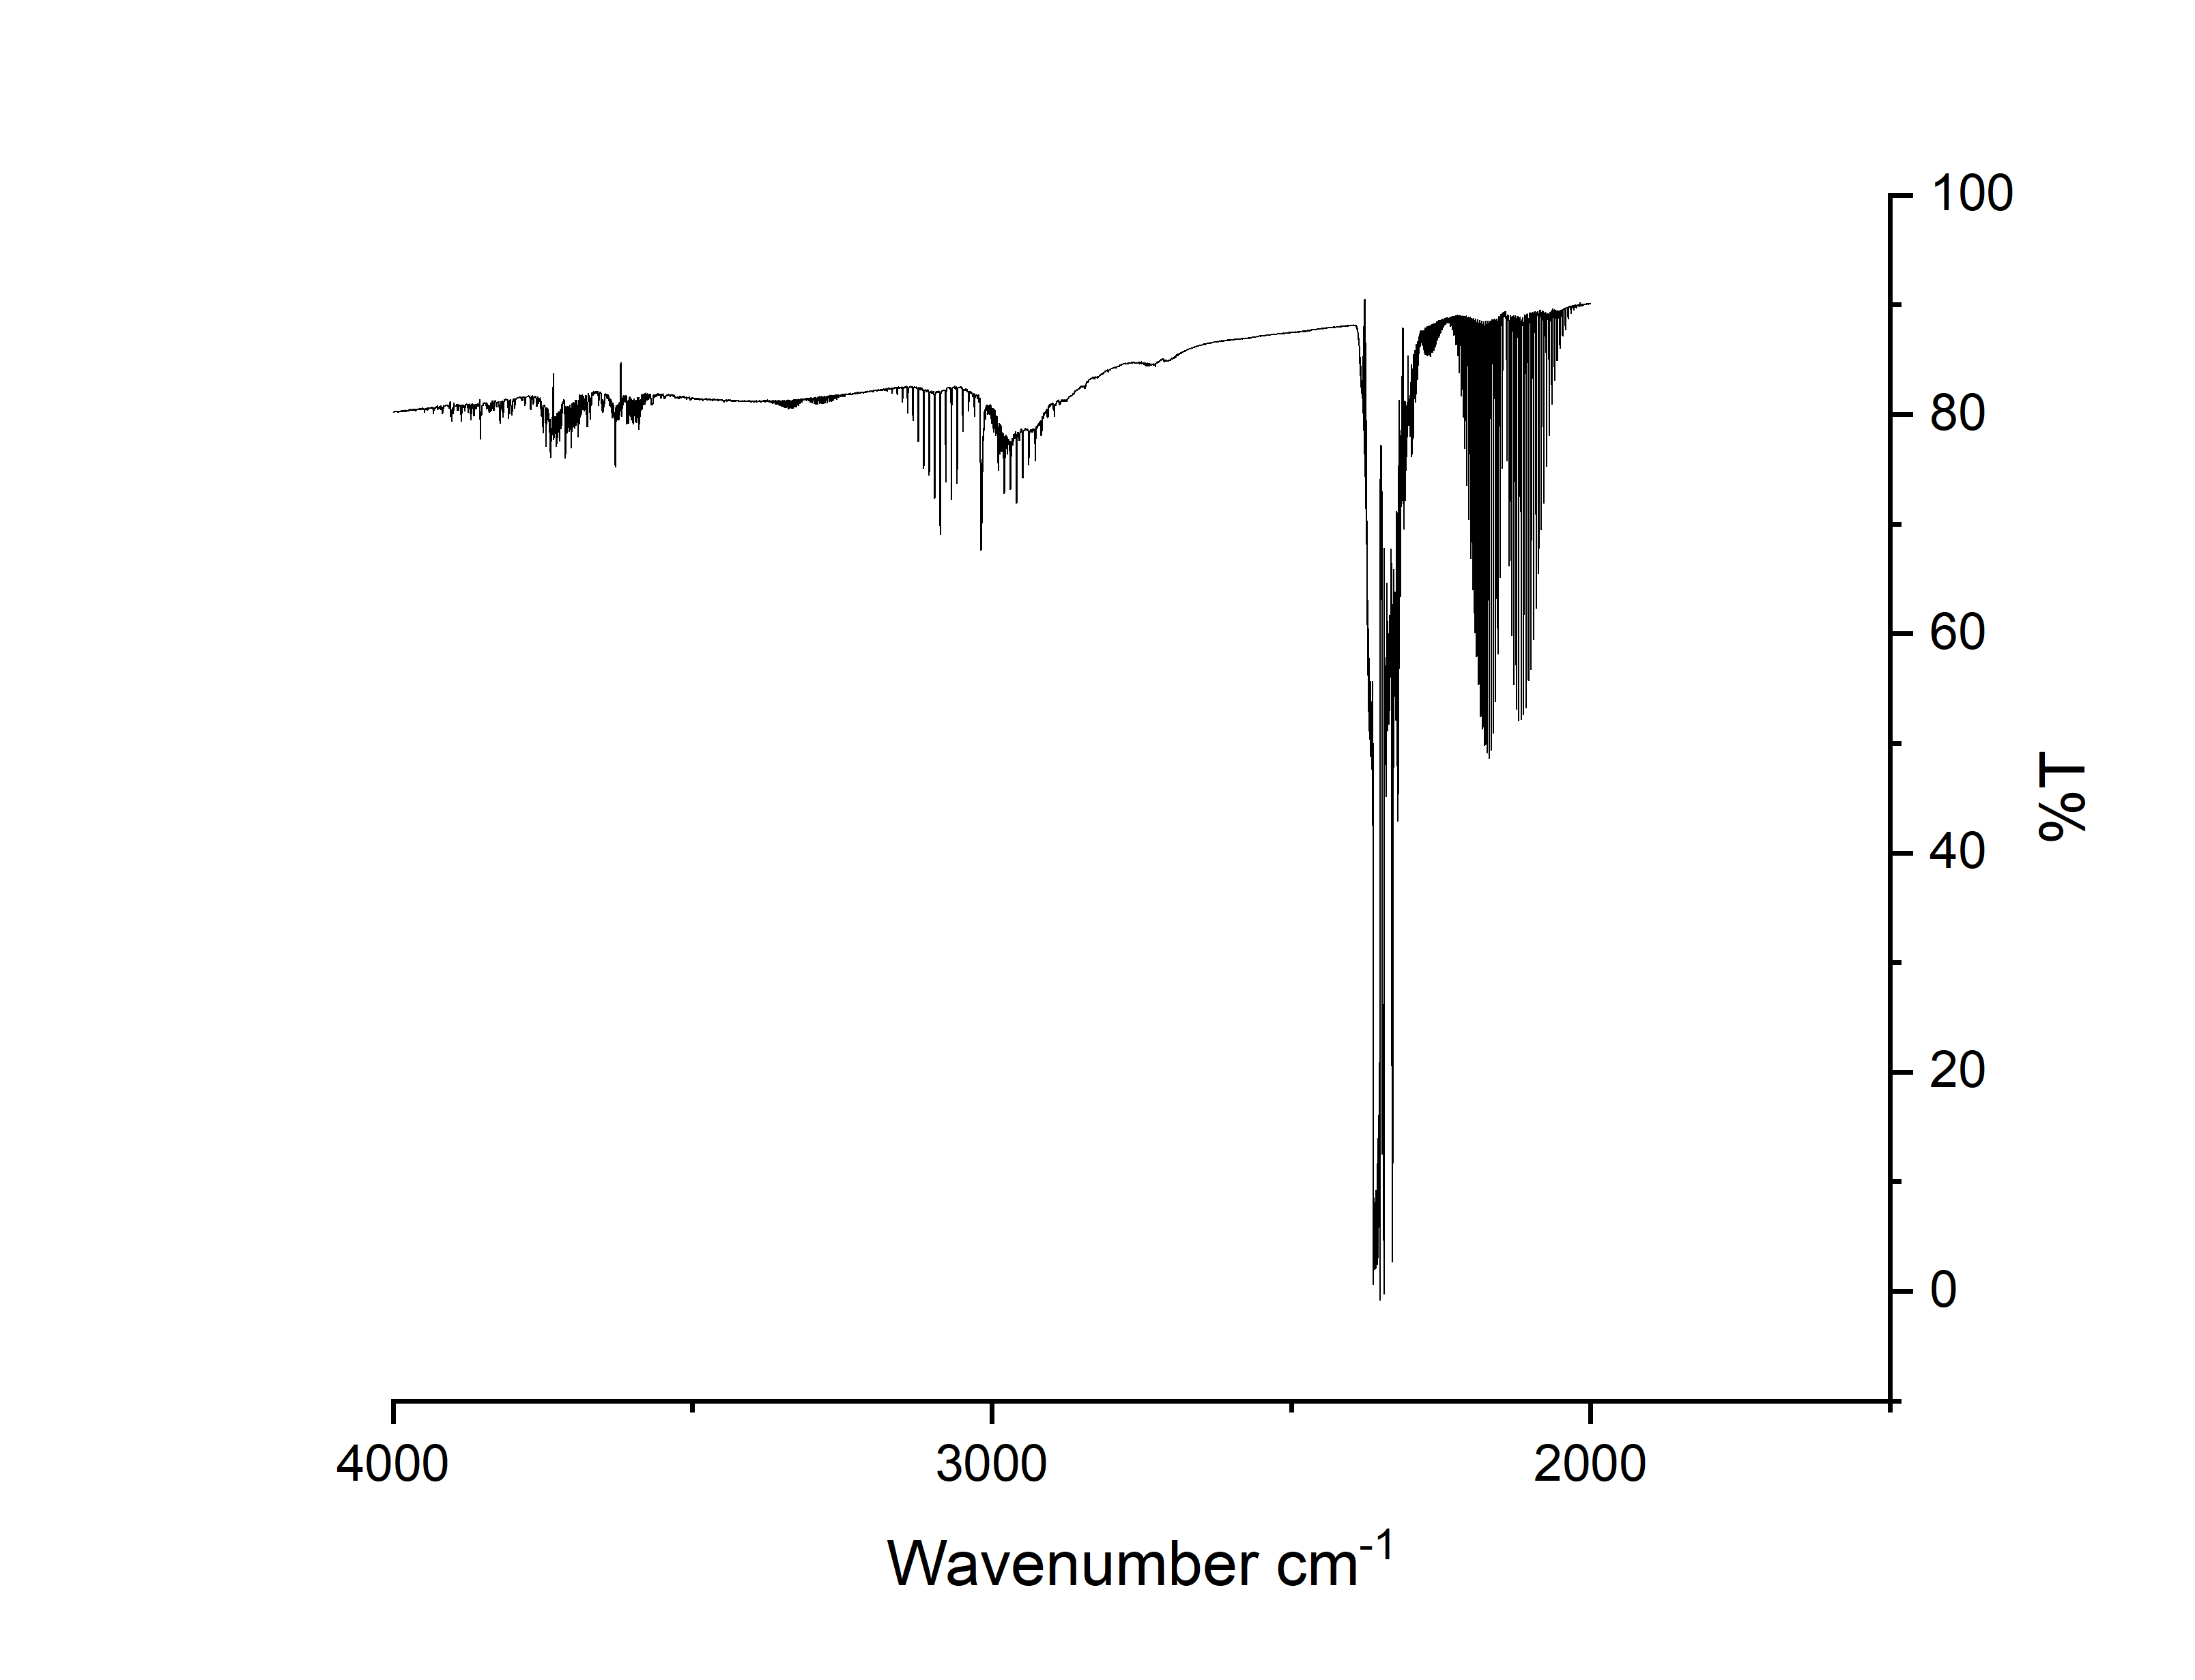
\includegraphics[width=\columnwidth]{Cig-all.png}
    \caption{The IR spectrum of the cigarette.}
    \label{cigall}
\end{figure}
\vspace{0.4in}

The peaks were compared to the literature values and different gases in the cigarette were identified. The peak at 2143.32 cm$^{-1}$ was identified as the fundamental absorption of CO as shown in Figure \ref{COfund}.

\begin{figure}[h!]
    \centering
    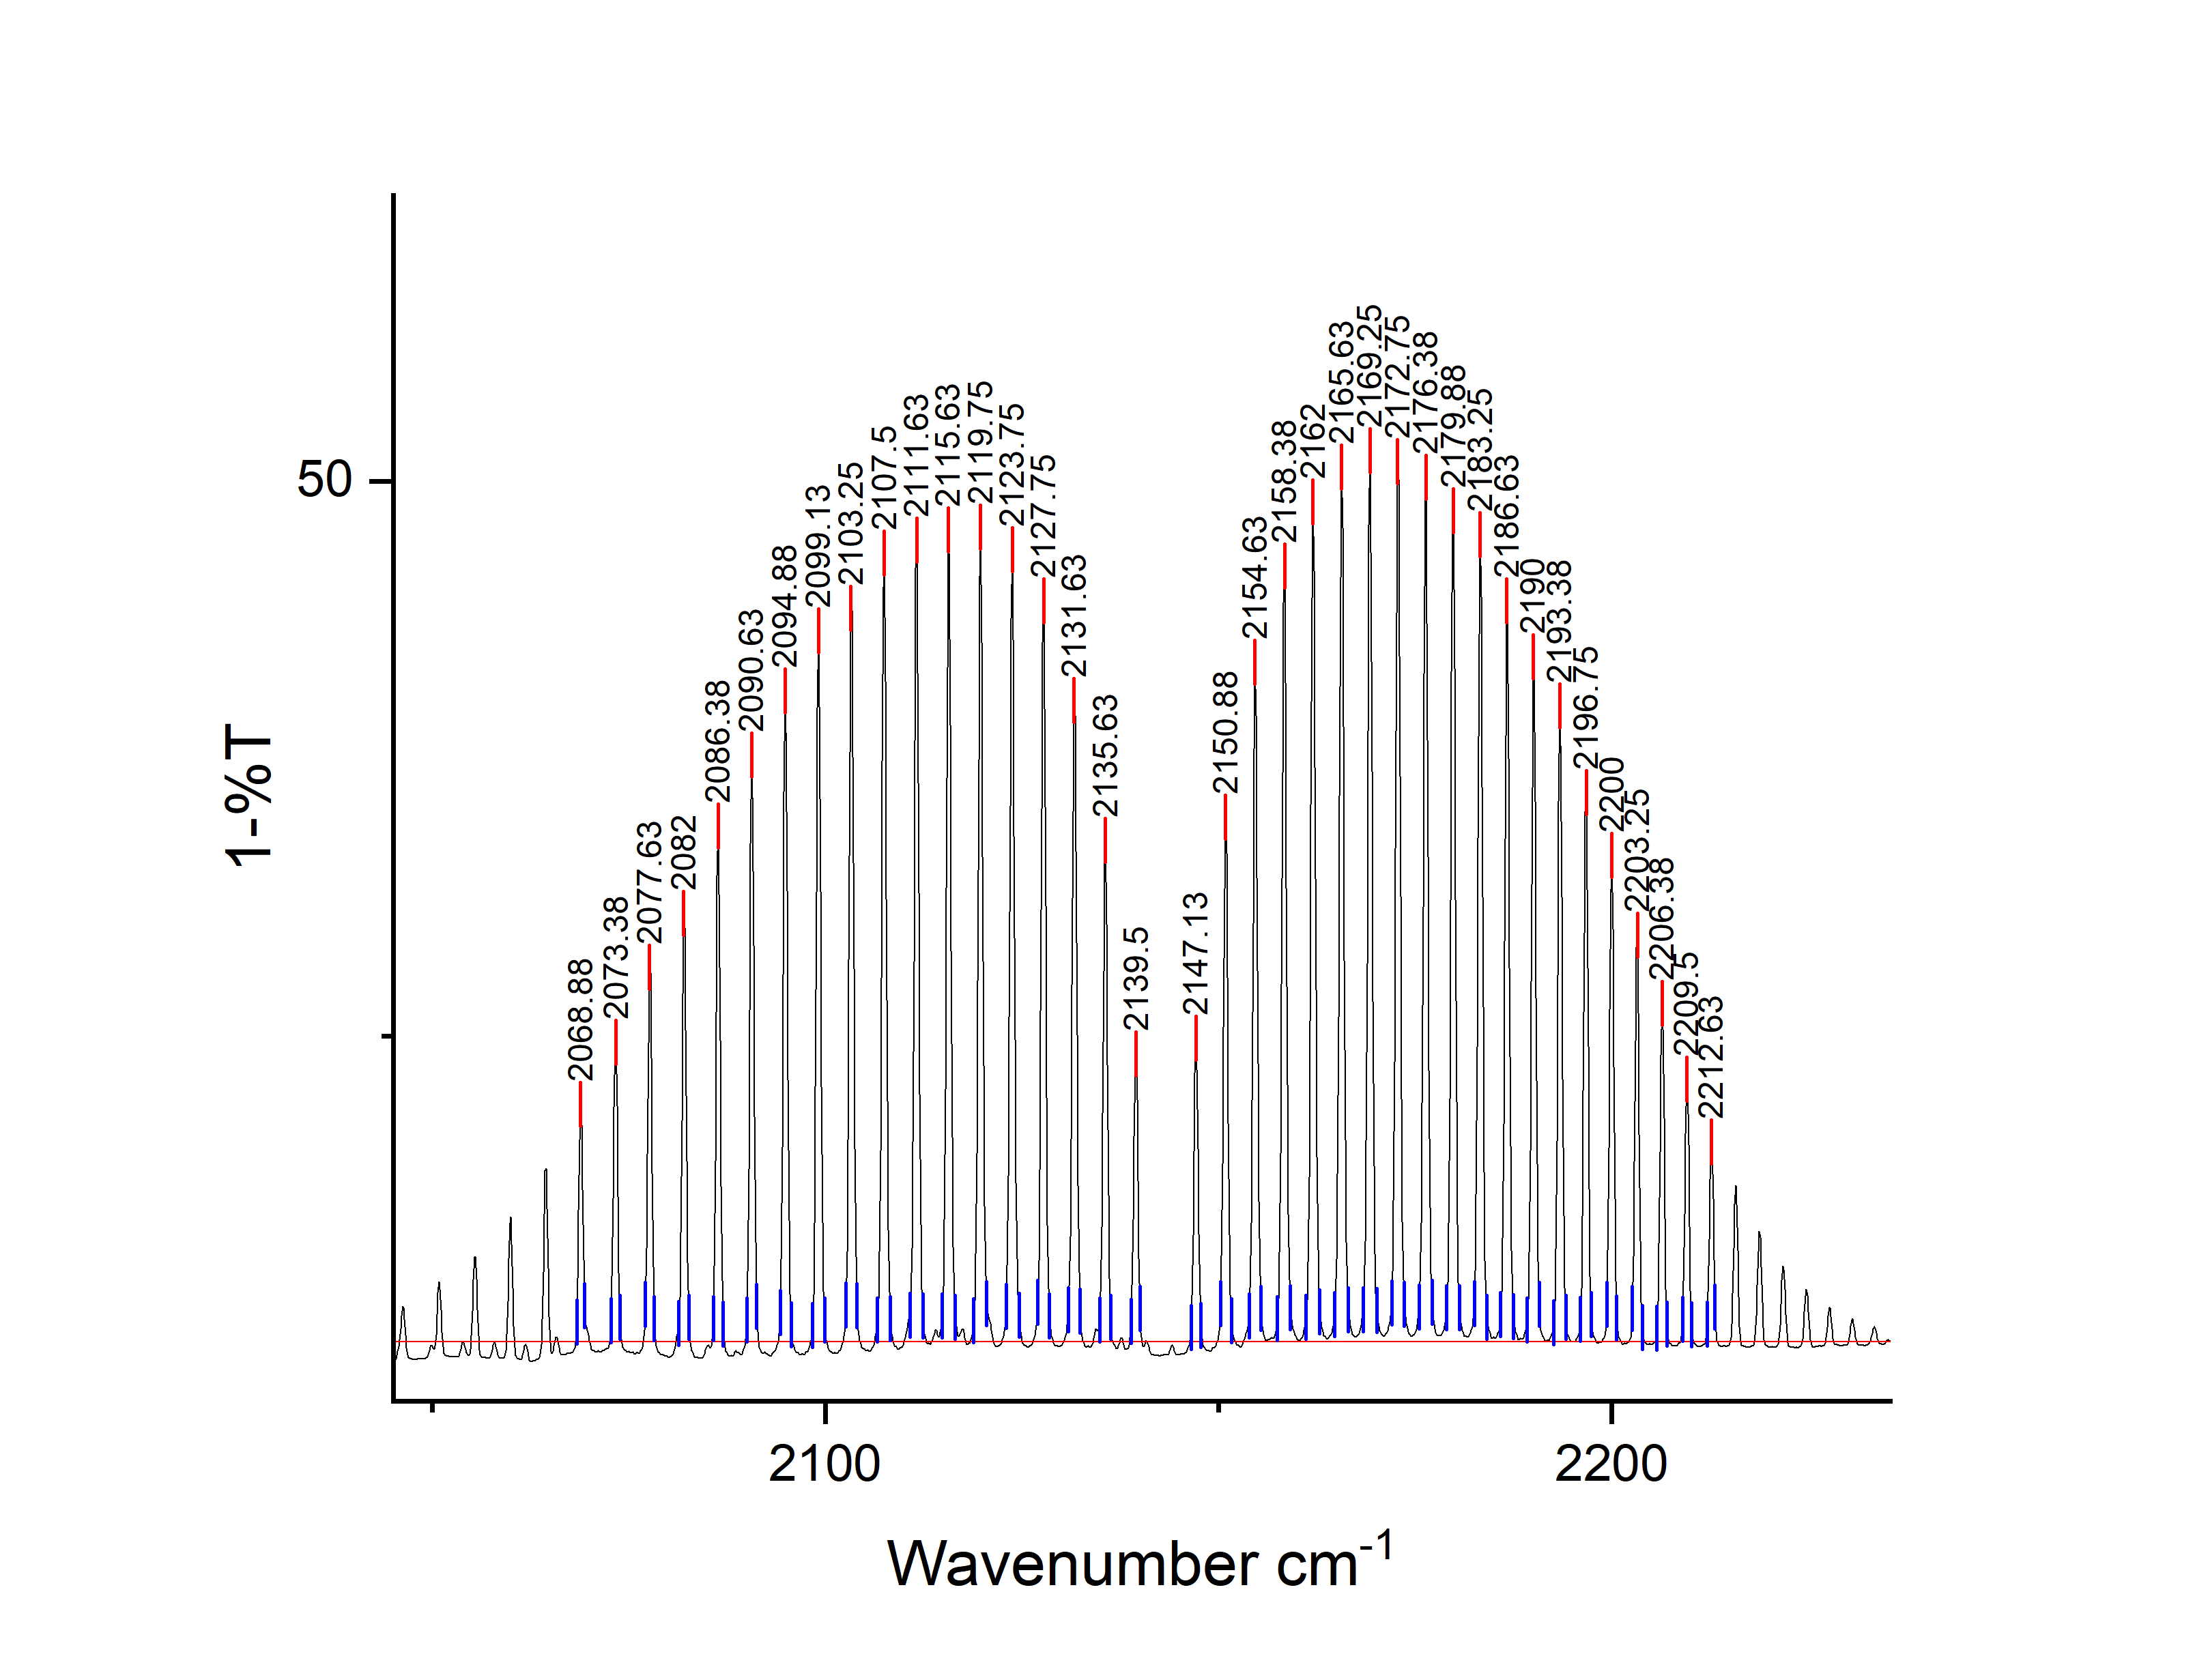
\includegraphics[width=\columnwidth]{CO-fundation.2.png}
    \caption{The IR spectrum of the fundamental absorption of CO.}
    \label{COfund}
\end{figure}
\vspace{0.4in}

The wavenumber of the fundamental absorption of the P-branch and R-branch for CO was recorded, and the value of R(J)-P(J) was calculated as shown in Table 5.  \\[3\baselineskip]

\begin{table}[h]
    \caption{The wavenumber of the fundamental absorption for HCl$^{37}$ in P branch and R branch.}
    \begin{tabular}{L{.1in}C{.7in}C{.7in}C{.7in}C{.8in}}\toprule
        J & P (cm$^{-1}$)      & R     (cm$^{-1}$)  & R(J)-P(J) (cm$^{-1}$)& R(J)-P(J+2) (cm$^{-1}$)\\\midrule
        0  & -       & 2147.13 & -     & 11.50 \\
        1  & 2139.50 & 2150.88 & 11.38 & 19.25 \\
        2  & 2135.63 & 2154.63 & 19.00 & 26.88 \\
        3  & 2131.63 & 2158.38 & 26.75 & 34.63 \\
        4  & 2127.75 & 2162.00 & 34.25 & 42.25 \\
        5  & 2123.75 & 2165.63 & 41.88 & 50.00 \\
        6  & 2119.75 & 2169.25 & 49.50 & 57.62 \\
        7  & 2115.63 & 2172.75 & 57.12 & 65.25 \\
        8  & 2111.63 & 2176.38 & 64.75 & 73.13 \\
        9  & 2107.50 & 2179.88 & 72.38 & 80.75 \\
        10 & 2103.25 & 2183.25 & 80.00 & -     \\
        11 & 2099.13 & -       & -     & -     \\\bottomrule
    \end{tabular}
\end{table}

\vspace{0.8in}

The peak at 4259.94 cm$^{-1}$ was identified as the first overtone of CO as shown in Figure \ref{COover}.\\[2\baselineskip]

\begin{figure}[h!]
    \centering
    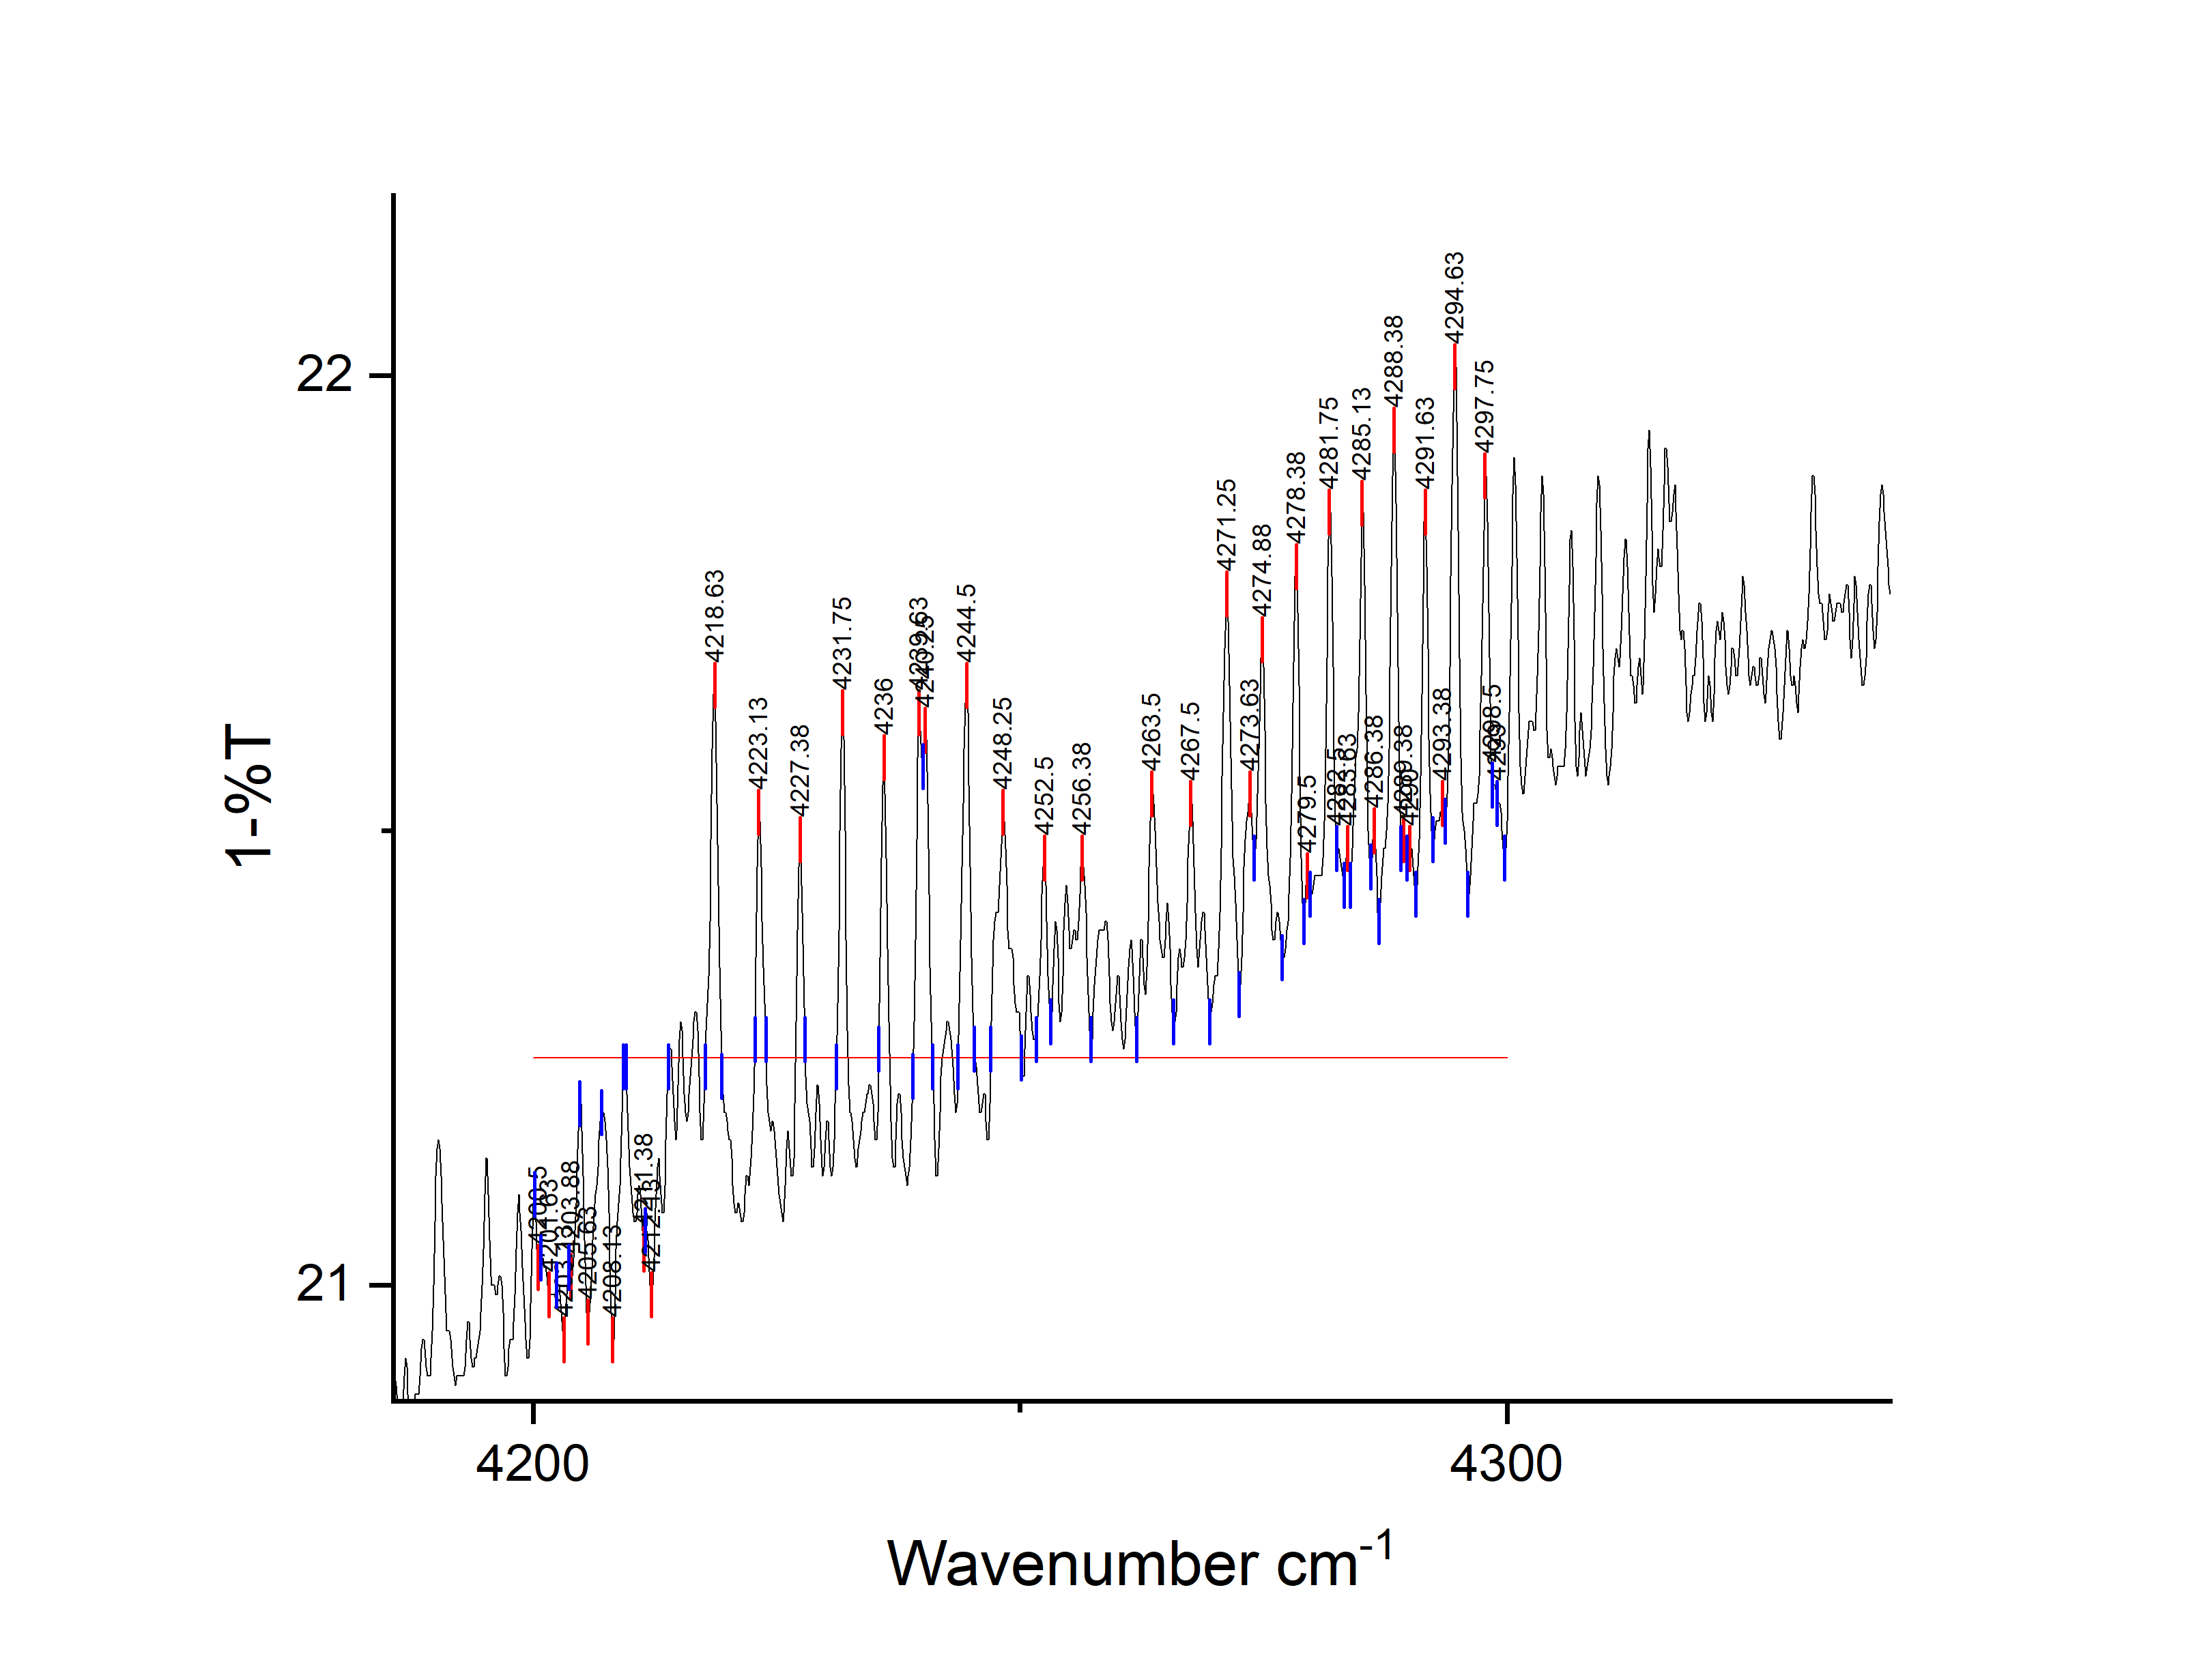
\includegraphics[width=\columnwidth]{CO-1st overtone.png}
    \caption{The IR sepctrum of the first overtone of CO.}
    \label{COover}
\end{figure}
\vspace{0.2in}


The value of $B_0$, $B_1$, $B_e$,$\alpha_e$, $r_0$, $r_1$, $r_e$, $\omega_e$, $x_e$, $G(0)$, and $k$ for CO were calculated using the same method as shown above, and the values were recorde and compared with the literature value as shown in Table 6. 

\begin{table}[h]
    \caption{The value of $B_0$, $B_1$, $B_e$,$\alpha_e$, $r_0$,$r_1$, $r_e$, $\omega_e$, $x_e$, $G(0)$, and $k$ for CO.}
    \begin{tabular}{L{0.9in}C{0.7in}C{0.7in}C{0.7in}}\toprule
          & Experimental data & Literature value & Error (\%) \\\midrule
        $B_0$ (cm$^{-1}$)& 1.9227 & 1.9293 \cite{CO-2} & 0.3\\
        $B_1$ (cm$^{-1}$)& 1.9053 & 1.9060 \cite{CO-2} & 0.04\\
        $B_e$ (cm$^{-1}$)& 1.9314 & 1.9381 \cite{CO-2}&0.3\\
        $\alpha_e$ (cm$^{-1}$)& 0.01744 & 0.017507 \cite{CO} &0.4\\
        $r_0$ (pm)& 113.3 & 113.03 \cite{CO-2} &0.2\\
        $r_1$ (pm)& 113.8 & 113.55\cite{CO-2} &0.2\\
        $r_e$ (pm)& 113.0 & - &-\\
        $\omega_e$ (cm$^{-1}$)& 2170.01 &  2169.8232 \cite{CO} &0.008\\
        $\omega_e x_e$ & 13.3450 & 13.2932 \cite{CO} & 0.4\\
        $x_e$ & 0.0061497 & - & - \\
        $G(0)$ (cm$^{-1}$)& 1081.67 & - &-\\
        $k$ (Nm$^{-1}$)& 1856.87 & 1860 \cite{HClbook} & 0.2\\\bottomrule
    \end{tabular}
\end{table}


% The results section should contain \textbf{all} the relevant experimental data that you collected.

%  %Here is an example of a table.
%  \begin{table}[h] %the [h] here instructs the table to assume a particular position on the page, read more on table positioning here: https://www.overleaf.com/learn/latex/Positioning_images_and_tables if your tables aren't positioned as you wish them to be, try experimenting with different parameters in the square brackets
%  \caption{Good header, or caption, makes the table or figure self-contained, it should provide enough information so that the table or figure could be understood on its own, without the main text.}
%  \begin{tabular}{L{.7in}C{.7in}C{.7in}C{.7in}}\toprule
%   & column 1 \textit{is really long} & column 2 & column 3\\\midrule
%  Line 1 & 68.28 & 45.30 & 56.79 \\
%  Line 2 & 54.06 & 38.63 & 46.35 \\\midrule %this is just an example on how to include an extra line, you can remove it if you do not need it
%  Line 3 & 61.17 & 41.97 & \\\bottomrule
%  \end{tabular}
%  \end{table}
%  %Be mindful that LaTeX -- unlike MS Word/Open Office/etc. -- does not allow for tables breaking across a page, by default. If the table is too big to fit into the remaining space of a page/column, it will instead be moved to the top of the following page/column. The resulting "empty" space will be filled with text, even if the text belongs to a different section! There are ways to prevent this, if you wish, but you may have to Google/look up how table formatting works :)

% Please organize the data in a logical manner, as this will make referencing from your discussion section much easier. You can see an example of what a table should look like in Table 1. Be mindful of formatting and presentation of both tables and figures; always consider the inclusion of textual cues, the placement of captions, correct units, overall appearance, and logical placement. Make sure your figures have good resolution! Grainy, unfocused, or otherwise shabby figures will lead to point deduction. Be careful about referencing, any literature data you use in your tables or figures needs to be cited. If you take a figure from a certain literature source, you need to \textbf{explicitly} reference it as such! Even if you make your own figures in ChemDraw or other software, if they are similar to or otherwise use ideas from a literature source, you must cite this appropriately.

%  Please make sure you describe the data, particularly any trends that are apparent -- always avoid data-dumps. The best result section will guide the reader through the data, pointing out any important trends, values, or possible errors.

%  \bigskip %this is a way to force LaTeX into inserting a blank line/space, can be small, medium, or fixed by instead using the '\vspace' command!

%  If you wish to learn more about how to format tables, please visit \href{https://es.overleaf.com/learn/latex/Tables}{\textbf{this page}}.
%  You can also find a handy tool which can generate tables for you here: \url{https://www.tablesgenerator.com/}




\section{Discussion}

%\hl{a short summary}

In this experiment, the vibrational-rotational spectrum of HCl and cigarette were obtained and analysed. The spectrum was recorded from 2000 cm$^{-1}$ to 6000 cm$^{-1}$ because the fundamental absorbing for a diatomic molecule was from 2000 cm$^{-1}$ to 4000 cm$^{-1}$, while the first overtone of a diatomic molecule was from 4000 cm$^{-1}$ to 6000 cm$^{-1}$. The resolution of the spectrometer was set to be 0.5, which was the highest value and would give a clear structure of the rotational spectrum as the energy absorbed for the rotational transition was small and could only be obtained if the resolution was high enough. 

The spectrums were obtained in a gas phase rather than a solution phase because the vibrational-rotational spectrum of a molecule in the gas phase was more clear and easier to analyse due to the high resolution. This was because the molecule in the gas phase would have more degree of freedom compared to the molecule in the solution phase. The molecules in the solution phase would have more interactions with the solvent molecules and were closer to each other, which results in less degree of freedom and low resolution. 

Before measuring HCl and cigarette gas, nitrogen was used as a background scan. This was because nitrogen was a diatomic molecule without a dipole moment when vibrating, meaning that it would not absorb any energy in the infrared region due to symmetry. Thus, nitrogen would not shown in the IR spectrum and would not affect the analysis of the sample. Besides, nitrogen was a relatively inert gas, which would not react with the sample. Therefore, nitrogen was an ideal gas for the background scan in this experiment. 

In the IR spectrum of HCl, each large peak of the fundamental absorption for HCl was followed by a smaller peak as shown in Figure 1. This was because Cl had an isotope $^{37}$Cl with an abundance 24.23\%, while $^{35}$Cl had an abundance as 75.77\%. Since $^{37}$ Cl was heavier than $^{35}$Cl, the reduced mass of HCl$^{37}$ was greater than the reduced mass of HCl$^{35}$. Therefore, the rotational constant (B) of HCl$^{37}$ would be lower than the rotational constant of HCl$^{35}$ because B was dependent on the reduced mass of the molecule based on equation 5. The energy absorption of HCl$^{37}$ would be lower than the energy absorption of HCl$^{35}$ based on equation 6. Therefore, the split peak with a smaller wavenumber would be the vibrational-rotational spectrum of HCl$^{37}$, while the split peak with a larger wavenumber would be the vibrational-rotational spectrum of HCl$^{35}$. 


The bond length of HCl$^{37}$ and HCl$^{35}$ were almost the same becaue $^{37}$Cl was an isotope of $^{35}$Cl, meaning that the chemical properties of $^{37}$Cl and $^{35}$Cl were similar. 

The equilibrium oscillation frequency, $\omega_e$, of HCl$^{37}$ was smaller than the equilibrium oscillation frequency of HCl$^{35}$ because $^{37}$Cl was heavier than $^{35}$Cl, resulting in slower vibration. 
This resulted in the smaller value of zero-point energy of HCl$^{37}$ than the zero-point energy of HCl$^{35}$ because the zero-point energy was dependent on the equilibrium oscillation frequency based on equation 2(a). 

The force constant of HCl$^{37}$ was slightly greater than the force constant of HCl$^{35}$ because the reduced mass of HCl$^{37}$ was greater than the reduced mass of HCl$^{35}$, resulting in greater force constant based on equation \ref{force constant}.

In the spectrum of cigarettes, each peak was identified as different gases in the cigarette and compared to the literature value as shown in Table \ref{cigarette}.

\begin{table}[h]
    \caption{The wavenumber of gases in the cigarette measured in the experiment and the literature value.}
    \begin{tabular}{L{.7in}C{.7in}C{.7in}C{.7in}}\toprule
        Gas & Experimental Data (cm$^{-1}$)      & Literature value (cm$^{-1}$)  & Error (\%) \\\midrule
        CO  & 2143.3 & 2143.7\cite{Cigarette} & 0.03 \\
        CO$_2$  & 2349.6 & 2349.3\cite{Cigarette} & 0.01 \\
        CH$_4$  &3017.6 &  3020.3\cite{Cigarette} & 0.09 \\
        HCN  & 3313.19 & 3311.5\cite{Cigarette} & 0.05 \\
        H$_2$O  & 3613.7 & - & - \\\bottomrule
    \end{tabular}
    \label{cigarette}
\end{table}


The experimental data was close to the literature value with a small error, which indicated that the experimental data was accurate. 

The rotational constant $B_v$ of CO was much smaller than the rotational constant of HCl. For a CO molecule, the difference between carbon and oxygen was small, meaning that the rotational center of the molecule would be close to the middle point of the two molecules. However, for an HCl molecule, the mass of chlorine was much larger than the mass of hydrogen, indicating that the rotational center of the molecule would be very close to chlorine. When the HCl molecule rotated, the chlorine atom would be almost static, while the hydrogen would rotate around the chlorine atom. 
The reduced mass of CO was much greater than the reduced mass of HCl. This resulted in the smaller rotational constant of CO than the rotational constant of HCl as the rotational constant depended on the reduced mass of the molecule based on equation 5. 



The bond length of the HCl was larger than the bond length of CO. This was because the bond length of a diatomic molecule was mainly dependent on the atomic radius of the two atoms. The atomic radius of chlorine was much larger than the atomic radius of oxygen and carbon because chlorine was in the third period and had one more electron shell filled with electrons, while oxygen and carbon were in the second period. Thus, the bond length of HCl would be greater than the bond length of CO.

The equilibrium oscillation frequency, $\omega_e$, of CO was smaller than the equilibrium oscillation frequency of HCl because hydrogen was much lighter than carbon and oxygen, resulting in faster vibration.

Since the value of $\omega_e$ of CO was smaller than the value of $\omega_e$ of HCl, the zero-point energy of CO was smaller than the zero-point energy of HCl based on equation 2(a).

The force constant of CO was much larger than the force constant of HCl because the reduced mass of CO was greater than the reduced mass of HCl, resulting in a larger force constant based on equation \ref{force constant}.

The calculated parameters for HCl$^{35}$, HCl$^{37}$, and CO were compared with the literature value as shown in Tables 3, 4, and 6. The error for each parameter was very small, which indicated that the experimental data was accurate. This might be due to the high resolution of the spectrum, which could give a clear structure of the spectrum and make the analysis of the spectrum more accurate.


In this experiment, one possible experimental error might be that the sample was not fully evaporated, which would lead to a lower resolution and might affect the analysis of the spectrum. This could be improved by increasing the time for waiting before starting to record the spectrum to ensure that the sample was fully evaporated. Another possible error would be that air might be introduced into the sample, and some molecules in the air might also shown in the spectrum which would affect the analysis of the spectrum. To limit the air introduced into the sample, the speed of adding the sample into the cell could be faster. 
During the recording of the spectrum for cigarettes, the sample might leak out of the sample cell, which would lead to a lower resolution, and gases with low concentrations might not be shown in the spectrum. This could be improved by ensuring that the sample was fully sealed before recording the spectrum.

This experimental setup could be used in industrial applications to identify the impurities in a sample as the vibrational-rotational spectrum of each molecule was unique. The spectrum could also be used to monitor the reaction process as the vibrational-rotational spectrum of the reactants and products were different. Therefore, the concentration of the reactants and products could be calculated respectively through the spectrum, which could reveal the reaction process. 

In this experiment, the vibrational-rotational spectrum of HCl and cigarette were obtained and analysed. The vibrational-rotational spectrum of HCl was split into two peaks due to the different isotopes of chlorine. The fundamental absorption of HCl$^{35}$ was 2885.76 cm$^{-1}$, while the fundamental absorption of HCl$^{37}$ was 2883.63 cm$^{-1}$. The first overtone of HCl$^{35}$ was 5663.50 cm$^{-1}$, while the first overtone of HCl$^{37}$ was 5667.57 cm$^{-1}$. The value of $B_0$, $B_1$, $B_e$, $\alpha_e$, $r_0$, $r_1$, $r_e$, $\omega_e$, $x_e$, $G(0)$, and $k$ for HCl$^{35}$ and HCl$^{37}$ were calculated and compared with the literature value. The vibrational-rotational spectrum of the cigarette was analysed and the gases in the cigarette were identified as CO, CO$_2$, CH$_4$, HCN, and H$_2$O. The wavenumber of each gas was compared to the literature value. The vibrational-rotational spectrum of CO was also analysed and the value of $B_0$, $B_1$, $B_e$, $\alpha_e$, $r_0$, $r_1$, $r_e$, $\omega_e$, $x_e$, $G(0)$, and $k$ for CO were calculated and compared with the literature value. The differences and trends of the parameters were discussed. The error for each parameter was very small, which indicated that the experimental data was accurate.

%  The ideal discussion will provide \textbf{full justification} of all the trends presented in the results section. 
%  Be sure to include complete reasoning for \textbf{why} the trends appear, make use of your knowledge of chemistry and concepts you explained in the introduction.
%  Reference the data tables from the results' section as necessary. 
%  %Here is an example of a figure.
%  \begin{figure}[h!]
%  \centering
%  \includegraphics[width=0.95\columnwidth]{figures/example.png} %an example of how to make your figure a specific size (fraction of the width of the column), if you'd like it to span the column instead, delete the number before the \)
%  \vspace{2mm} %just an example of how space can be added if need be, replace with '\hspace' for horizontal padding
%  \caption{Same as with table headers applies here. Please note that while in tables the caption is placed above, with figures the caption should be placed below.}
%  \end{figure}

%  Make use of figures and/or external references to support your discussion points. An example figure is shown above as Figure 1.

%  The best discussion will also include a brief paragraph with conclusions (for each part of the experiment) and future work. Future work, in this case, refers to a brief discussion on the validity of your chosen method, and the justification of using computational methods for the purposes of this experiment. The best discussion will offer some suggestions on the improvement of the experimental design.

%  \textbf{Please use concise and scientific tone in your writing. Academic writing, by convention, uses the past tense and a passive voice. Try to emulate the style you see in textbooks/papers. Avoid the use of first (I/we) or second (you) person, informal language, overuse of conjunctions and pronouns (especially 'this/that'). Make sure to proofread and spellcheck your work before submitting!}

%  Again, if you aren't sure what is appropriate for academic writing, please consult the many guides available online, such as \href{https://libguides.reading.ac.uk/writing/style}{\textbf{this one}}





\section{Investigation Question}

%this is a citation \cite{Example}

In the industrial, FTIR could give information about complete and incomplete combustion, which would be discussed below. 

During the complete combustion, the fuel would be fully oxidized to carbon dioxide and water as shown in equation \ref{complete}. 

\begin{equation}
    C_xH_y + O_2 \rightarrow CO_2 + H_2O
    \label{complete}
\end{equation}

The fuel usually not only contained carbon and hydrogen, but also contained other elements such as nitrogen, sulfur, and oxygen. Thus, nitrogen dioxide might also be produced during the complete combustion.\cite{NOx}.

If the combustion was incomplete, carbon monoxide would be produced instead of carbon dioxide, and other nitrogen oxides (NO$_x$) might also exist.\cite{NOx} Methane was also an important product during the incomplete combustion as shown in the equation. \cite{PCFC}

The sample after combustion could be analysed using FTIR. The representative peaks in the spectrum could be identified as compared to the literature value. 
The peak from 2200 cm$^{-1}$ to 2400 cm$^{-1}$ represented carbon dioxide, while the peak from 2000 $cm^{-1}$ to 2200 $cm^{-1}$ represented carbon monoxide. Peaks from 2300 cm$^{-1}$ to 3000 cm$^{-1}$ could be assigned to aliphatic carbons.\cite{FTIR} The fundamental absorption of OH strech for H$_2$O was around 3500 cm$^{-1}$.\cite{H2O} The peak around 3020.3 cm$^{-1}$ was correspond to CH$_4$.\cite{Cigarette} 

The main difference between complete and incomplete combustion was the production of carbon dioxide or carbon monoxide. Therefore, the analysis could focus on the amount of carbon dioxide and carbon monoxide. The concentration of the gases could be determined using the peak area of the fundamental absorption based on the Beer-Lambert law as shown in equation \ref{Beer-Lambert}.\cite{beer}

\begin{equation}
    A = \epsilon cl
    \label{Beer-Lambert}
\end{equation}

The ratio of carbon dioxide and carbon monoxide could be calculated by knowing the concentration of both gases, which could be used to determine whether the combustion was complete or incomplete.

This experiment could reveal the concentration of carbon dioxide, which was the main product of complete combustion, and carbon monoxide, which was the main product of incomplete combustion. Thus, it could monitor the process of combustion. The combustion would tend to be complete if the temperature increased. Therefore, this experiment could also be used to determine at which temperature the combustion was fully complete.\cite{FTIR} However, if there were too many gases in the sample, the spectrum might be too complicated to analyse. Besides, this experiment could only measure gas but not liquid or solid, and also the gas without dipole moment would not shown in the spectrum as well. However, during incomplete combustion, carbon might also form, which could not be shown in the spectrum. Therefore, this experiment could only be used to measure the gas with dipole moment. The carbon dioxide might also be produced during incomplete combustion, which might be difficult to analyse. 

To improve the reliability of the results, TGA-FTIR could be used.\cite{TGA} Another method called PCFC-FTIR was also an alternative method to improve the reliability of the results.\cite{PCFC}



% \begin{figure}[h!]
%     \centering
%     \includegraphics[width=\columnwidth]{CO2.png}
%     \caption{The vibrational-rotational spectrum of carbon dioxide.}
%     \label{CO2}
% \end{figure}





% Please include the write-up to your investigation question here. Include any relevant figures, sources, or background information, as instructed in your manual.
% \\
% The best Investigation Question will include:
% \\1) a short, relevant introduction to the problem,
% \\2) a clear and well-worded proposal of a solution (hypothesis), and 
% \\3) a concise and well-researched backing/explanation for the solution. 

% Use appropriate scientific language and make sure to properly reference all of your sources!

% \vspace{8mm}
% \hrule

% %% THE FOLLOWING SECTIONS CONTAIN SOME ADDITIONAL INFORMATION FOR YOUR CONVENIENCE, MAKE SURE TO REMOVE THEM FROM YOUR OWN REPORT %%

% \section*{Note on the Citation} %Delete this section in your own report
% All sources should be formatted in the Royal Society of Chemistry (RSC) referencing style \cite{Example}. If you don't know what this means, I strongly recommend reviewing how citation and referencing works in general, and looking into the style guides for the RSC style in particular. 
% %more info at https://edu.rsc.org/download?ac=14556  

% If you use a different referencing style (MLA, Harward, etc.) please indicate so in a footnote\footnote{Example on how to format a footnote in \LaTeX{}} of your citation section, so that the demonstrator marking your work knows that you've used something different and can check it for errors!

% With Overleaf, you can simply import a .bib file into your file tree (the panel on the left-most side of your screen) and the bibliography command will automatically compile them for you. Please make sure to include relevant in-text references using the \textbackslash cite command.
% The \textbackslash printbibliography command will then generate the proper references section for you!

% .bib file can be easily obtained using a reference-management software. If you don't know what this is, or don't yet use one, I \textbf{strongly} recommend looking into one! Personally, I use \href{https://www.mendeley.com/reference-management/reference-manager}{Mendeley}, which has both a desktop version and a browser plug-in — this enables you to add references as you browse/research. If you learn how to use a reference management software now, it will save you tons of time later on; while you're writing your thesis, or other works in the future.

% Further guidelines on referencing in LaTeX can be found here:
% \url{https://www.overleaf.com/learn/latex/Bibliography\_management\_in\_LaTeX}

% \section*{Tips and Tricks} %make sure to delete this from your report!!

% \LaTeX{} is a widely used compiler, there are hundreds of tutorial articles and videos online - please make use of them! Google is your friend, you need only ask.

% % Sidenote from Angie: I'm (a bit) sorry for bullying you with Overleaf and LaTeX coding, but I promise if you give it a chance, you'll learn to love it :) it's very useful for writing larger pieces of academic writing ⁠— such as your future thesis! Plus, it is another shiny, new skill to spruce up your future CVs.

% \subsection*{How to write Mathematics} %make sure to delete this from your report

% \LaTeX{} is great at typesetting mathematics. Let $X_1, X_2, \ldots,
% X_n$ be a sequence of independent and identically distributed random
% variables with $\text{E}[X_i] = \mu$ and $\text{Var}[X_i] = \sigma^2 <
% \infty$, and let
% \[S_n = \frac{X_1 + X_2 + \cdots + X_n}{n}
%       = \frac{1}{n}\sum_{i}^{n} X_i\]
% denote their mean. Then as $n$ approaches infinity, the random
% variables $\sqrt{n}(S_n - \mu)$ converge in distribution to a normal
% $\mathcal{N}(0, \sigma^2)$.

% \subsection*{How to add Lists} %make sure to delete this from your report

% You can make lists with automatic numbering \dots

% \begin{enumerate} %for numbered list
% \item Like this,
% \item and like this.
% \end{enumerate}
% \dots or like this, \dots
% \begin{itemize} %for bullet points
% \item Like this,
% \item and like this.
% \end{itemize}


%% I M P O R T A N T %%
%%!!!REFERENCES -- REVIEW FOR YOUR OWN REPORT!!!%%

\bibliography{ref} %This command generates your bibliography. PLEASE MAKE SURE TO CHANGE THE NAME IN THESE CURLY BRACKETS TO WHATEVER YOUR .BIB FILE IS CALLED!!
\bibliographystyle{rsc} %setting for the RSC's .bst (style) file -- do NOT change this, unless you wish to define a new citation style

\end{document}


%Best of luck with your report! 

%Last SideNote: If you have any questions ask them during the lab session, you should have plenty of time and opportunity to go over everything. If you need more help once your sessions are over and you can't figure something out yourself, you can contact me at angie.matusova@ed.ac.uk. Please, don't hesitate to get in touch if you're struggling with something (though, please make sure you've exhausted all the other options before contacting me; i.e. you've reviewed all the material available on Learn and/or tried looking up your query online).